% Inspired by Bùi Vân Anh
% Begin rewrite by ledangquangdangquang on 2024-09-30
\documentclass{thesis-config}

%----- PERSONAL INFORMATION -----
\title{Mô phỏng kênh MIMO băng rộng sử dụng biểu diễn DPS}
\author{LÊ ĐĂNG QUANG}
\specialization{Ngành KT Điện tử \& Viễn thông}
\authoremail{quang.ld224113@sis.hust.edu.vn}
\universitycity{HÀ NỘI}
\university{ĐẠI HỌC BÁCH KHOA HÀ NỘI}
\school{Điện - Điện tử}
\department{}
\advisor{TS. Nguyễn Hồng Anh}
\degree{Đồ án tốt nghiệp}
\degreemonth{\the\month}
\degreeyear{\the\year}
\major{}

%----- MAIN DOCUMENT -----
\begin{document}
    % MỞ ĐẦU 
    \input{MoDau/Bia} 
    % NHIỆM VỤ ĐỒ ÁN TỐT NGHIỆP
% Bảng thông tin
\noindent
\begin{tabularx}{\textwidth}{>{\centering\arraybackslash}X>{\centering\arraybackslash}X}
    BỘ GIÁO DỤC \& ĐÀO TẠO & \textbf{CỘNG HÒA XÃ HỘI CHỦ NGHĨA VIỆT NAM} \\
    \textbf{ĐẠI HỌC BÁCH KHOA HÀ NỘI} & \textbf{Độc lập - Tự do - Hạnh phúc} \\
\end{tabularx}

\begin{center}
    \textbf{\centering NHIỆM VỤ\\}
    \textbf{\centering ĐỒ ÁN TỐT NGHIỆP\\}
\end{center}

{\centering Họ và tên sinh viên: \dotfill \\}
{\centering\makebox[\linewidth]{Khoa:\dotfill Viện:\dotfill Ngành:\dotfill}}
\textit{ % Bên trong in nghiêng
    \begin{enumerate}
        \item Tên đề tài:\\ .\dotfill
        \item Nội dung đề tài:\\ .\dotfill\\ .\dotfill\\ .\dotfill\\ .\dotfill\\ .\dotfill\\ .\dotfill\\ .\dotfill
        \item Cán bộ hướng dẫn:\\ \makebox[\linewidth]{Phần \hspace{7cm}  Họ tên cán bộ} \\  .\dotfill\\ .\dotfill\\ .\dotfill\\ .\dotfill
        \item Thời gian giao đề tài:\dotfill
        \item Thời gian hoàn thành đề tài:\dotfill
    \end{enumerate}
}
% Ngày tháng năm
\begin{flushleft}
    Ngày \makebox[1cm]{\dotfill} tháng \makebox[1cm]{\dotfill} năm \makebox{2024} \\
\end{flushleft}
\noindent
\begin{tabularx}{\textwidth}{>{\centering\arraybackslash}X>{\centering\arraybackslash}X}
    \textbf{LÃNH ĐẠO BỘ MÔN} & \textbf{CÁN BỘ HƯỚNG DẪN}
\end{tabularx}

\vspace{1.5cm}
\begin{center}
    \textbf{SINH VIÊN THỰC HIỆN\\}
    \textit{{(Ký và ghi rõ họ tên)}}
\end{center}
\thispagestyle{empty}
\cleardoublepage
 
    \thispagestyle{empty}

\subsection*{\centering Lời cảm ơn}

Em xin gửi lời cảm ơn chân thành tới TS. Nguyễn Hồng Anh đã định hướng, góp ý và hỗ trợ em trong quá trình thực hiện đồ án tốt nghiệp. Những trao đổi về mô hình kênh MIMO, phương pháp biểu diễn DPS và cách kiểm chứng bằng mô phỏng đã giúp em hoàn thiện hơn cả phần lý thuyết lẫn phần triển khai MATLAB.

Em cũng xin cảm ơn các thầy cô Trường Điện -- Điện tử, Đại học Bách khoa Hà Nội đã trang bị cho em nền tảng kiến thức trong suốt quá trình học tập. Cuối cùng, em xin cảm ơn gia đình và bạn bè đã luôn động viên, tạo điều kiện để em hoàn thành đồ án này.

\subsection*{\centering Tóm tắt nội dung đồ án}

Đồ án nghiên cứu bài toán mô phỏng kênh MIMO băng rộng dựa trên mô hình kênh hình học. Trong mô hình này, kênh được biểu diễn dưới dạng tổng các hàm mũ phức (SoCE) của nhiều thành phần đa đường. Cách biểu diễn SoCE có ý nghĩa vật lý rõ ràng, nhưng chi phí tính toán tăng theo số mẫu thời gian, số điểm tần số, số anten và số MPC.

Để giảm độ phức tạp, đồ án khai thác đặc điểm kênh bị giới hạn băng theo các chiều Doppler, trễ, góc phát và góc thu. Trên cơ sở đó, chuỗi prolate spheroidal rời rạc (DPS) được sử dụng để biểu diễn khối kênh trong một không gian con có số chiều nhỏ hơn. Phần mô phỏng được triển khai bằng MATLAB với bốn nhánh: SoCE tham chiếu, DPS chính xác, DPS xấp xỉ 4D và phương pháp hybrid kết hợp DPS theo thời gian--tần số với hàm mũ không gian trực tiếp.

Trong cấu hình mô phỏng hiện tại, phương pháp hybrid đạt NMSE \(4{,}29\times10^{-7}\) so với SoCE tham chiếu, trong khi DPS chính xác đạt NMSE \(8{,}53\times10^{-9}\). Các kết quả này cho thấy biểu diễn DPS có thể giảm số chiều tính toán trong phạm vi cấu hình đang xét, đồng thời vẫn giữ sai số nhỏ. Hướng phát triển tiếp theo là quét tham số DPS, mở rộng kích thước mô phỏng và tái tạo một kết quả định lượng cụ thể trong bài báo gốc.

\vfill
\begin{tabularx}{\textwidth}{>{\centering\arraybackslash}X>{\centering\arraybackslash}X}
    \centering
    & Sinh viên thực hiện \\
    \centering
    &\fontsize{10pt}{0}\selectfont Ký và ghi rõ họ tên \\
    \centering
\end{tabularx}
  
\cleardoublepage
 
    \input{MoDau/MucLuc} 
    \pagenumbering{roman} % Đánh số trang thứ tự la mã
    \phantomsection\section*{\centering DANH MỤC KÝ HIỆU VÀ CHỮ VIẾT TẮT}
\addcontentsline{toc}{section}{\numberline {} DANH MỤC KÝ HIỆU VÀ CHỮ VIẾT TẮT}
\small
\setlength{\tabcolsep}{4pt}
\begin{tabularx}{\textwidth}{@{}p{0.13\textwidth} X@{}}
    \toprule
    Ký hiệu & Ý nghĩa \\
    \midrule
    AoA & Góc tới (Angle of Arrival) \\
    AoD & Góc khởi hành (Angle of Departure) \\
    DPS & Chuỗi prolate spheroidal rời rạc (Discrete Prolate Spheroidal Sequences) \\
    DPSS & Cách viết khác của DPS trong một số tài liệu \\
    GCM & Mô hình kênh dựa trên hình học (Geometry-based Channel Model) \\
    MIMO & Hệ thống nhiều anten phát và thu (Multiple-Input Multiple-Output) \\
    MPC & Thành phần đa đường (Multipath Component) \\
    MSE & Sai số bình phương trung bình (Mean Squared Error) \\
    NMSE & Sai số bình phương trung bình chuẩn hóa (Normalized Mean Squared Error) \\
    Rx & Phía thu (Receiver) \\
    SoCE & Tổng các hàm mũ phức (Sum of Complex Exponentials) \\
    Tx & Phía phát (Transmitter) \\
    ULA & Mảng tuyến tính đều (Uniform Linear Array) \\
    \bottomrule
\end{tabularx}
\normalsize
\cleardoublepage
 
    \input{MoDau/DanhMucHinhVe} 
    \input{MoDau/DanhMucBangBieu} 
    \pagenumbering{arabic}% Đánh số trang thứ tự bình thường
    % NỘI DUNG
    \chaptercustom{1}{ĐẶT VẤN ĐỀ VÀ LÝ DO SỬ DỤNG DPS}
\setcounter{section}{1}
\label{chap:problem_dps}

\subsection{Bối cảnh mô phỏng kênh MIMO băng rộng}
\label{subsec:ch1_context}

Mô phỏng kênh truyền là một bước quan trọng trong quá trình thiết kế và đánh giá hệ thống thông tin vô tuyến. Kênh truyền mô tả sự biến đổi của tín hiệu từ phía phát đến phía thu; đáp ứng kênh là đại lượng toán học dùng để biểu diễn sự biến đổi đó. Trước khi triển khai thuật toán trên phần cứng hoặc kiểm chứng bằng đo đạc thực tế, mô phỏng cho phép khảo sát ảnh hưởng của hiện tượng đa đường, dịch Doppler, trải trễ và cấu trúc anten đến đáp ứng kênh.

Đồ án xét hệ thống nhiều anten phát và nhiều anten thu (Multiple-Input Multiple-Output, MIMO) hoạt động trên một dải tần gồm nhiều điểm tần số. Trong hệ thống này, mỗi cặp anten phát--thu có một đáp ứng kênh riêng. Đồng thời, chuyển động của thiết bị làm đáp ứng kênh thay đổi theo thời gian, còn hiện tượng đa đường làm đáp ứng khác nhau giữa các điểm tần số. Vì vậy, một khối kênh MIMO băng rộng phải được mô tả đồng thời theo bốn chiều: thời gian, tần số, anten phát và anten thu.

Một mô hình thường được sử dụng cho bài toán này là mô hình kênh dựa trên hình học (Geometry-based Channel Model, GCM). Trong GCM, tín hiệu đến máy thu qua nhiều đường lan truyền do phản xạ, nhiễu xạ hoặc tán xạ. Đóng góp của mỗi đường được mô tả bằng một thành phần đa đường (Multipath Component, MPC). Mỗi MPC mang các tham số vật lý như trọng số phức, dịch Doppler, trễ truyền, góc khởi hành và góc tới. Khi lấy tổng đóng góp của các MPC, đáp ứng kênh có dạng tổng các hàm mũ phức (Sum of Complex Exponentials, SoCE) như trong bài báo của Kaltenberger và cộng sự \cite{Kaltenberger2007}.

SoCE giữ được mối liên hệ trực tiếp giữa đáp ứng kênh và các đường lan truyền, nhưng cách tính này có thể đòi hỏi nhiều phép toán. Khi số MPC, số mẫu thời gian, số điểm tần số và số anten tăng, đóng góp của từng MPC phải được tính tại ngày càng nhiều điểm của khối kênh. Vì vậy, vấn đề chính của đồ án là tìm một cách biểu diễn có khả năng giảm khối lượng tính toán, đồng thời duy trì sai số xấp xỉ trong phạm vi kiểm soát.

\subsection{SoCE và nút thắt tính toán}
\label{subsec:ch1_soce_bottleneck}

Để thực hiện mô phỏng trên máy tính, các biến liên tục của mô hình được lấy mẫu. Sau khi rời rạc hóa theo thời gian, tần số và vị trí anten, đáp ứng kênh MIMO băng rộng có thể viết gọn dưới dạng SoCE đa chiều:
\begin{equation}
h_{\mathbf{m}}
= \sum_{p=0}^{P-1}\eta_p e^{j2\pi\mathbf{f}_p^T\mathbf{m}}.
\label{eq:ch1_soc_compact}
\end{equation}
Trong đó, \(\mathbf{m}\) là véc-tơ chỉ số xác định một điểm trong khối kênh, gồm chỉ số thời gian, tần số, anten phát và anten thu; \(\mathbf{f}_p\) là véc-tơ chứa các tần số chuẩn hóa tương ứng của MPC thứ \(p\); \(\eta_p\) là trọng số phức biểu diễn biên độ và pha của MPC đó; còn \(P\) là tổng số MPC. Tích vô hướng \(\mathbf{f}_p^T\mathbf{m}\) gộp sự biến thiên theo bốn chiều vào một số hạng pha. Dấu pha và cách chuẩn hóa cụ thể của từng chiều được trình bày tại Chương 3.

Với cách tính trực tiếp, tại mỗi điểm mẫu \(\mathbf{m}\), biểu thức \eqref{eq:ch1_soc_compact} cần cộng đóng góp của toàn bộ \(P\) MPC. Nếu khối mô phỏng có \(M\) mẫu thời gian, \(Q\) điểm tần số, \(N_{\mathrm{Tx}}\) anten phát và \(N_{\mathrm{Rx}}\) anten thu, bậc độ phức tạp có thể viết:
\begin{equation}
C_{\mathrm{SoCE}}
= \mathcal{O}\!\left(MQN_{\mathrm{Tx}}N_{\mathrm{Rx}}P\right).
\label{eq:ch1_soce_complexity}
\end{equation}
Ký hiệu \(\mathcal{O}(\cdot)\) trong \eqref{eq:ch1_soce_complexity} mô tả xu hướng tăng của khối lượng tính toán, không phải thời gian chạy tuyệt đối. Biểu thức này cho thấy chi phí của SoCE trực tiếp tăng theo tích của số mẫu trong bốn chiều và số MPC. Đây là điểm bất lợi đáng chú ý trong các mô phỏng cần khảo sát nhiều cấu hình tham số hoặc hướng tới xử lý thời gian thực. Chương 2 sẽ phân tích chi tiết hơn số phép tính của SoCE và DPS sau khi giới thiệu vai trò của không gian con DPS.

\subsection{Cấu trúc giới hạn băng của kênh}
\label{subsec:ch1_bandlimited}

Mặc dù SoCE trực tiếp có chi phí lớn, kênh trong \eqref{eq:ch1_soc_compact} không phải là một tín hiệu tùy ý. Các thành phần của véc-tơ \(\mathbf{f}_p\) bị ràng buộc bởi những đại lượng vật lý của hệ thống. Cụ thể, vận tốc cực đại giới hạn dịch Doppler; phạm vi trễ của các đường truyền giới hạn tần số chuẩn hóa theo chiều tần số; còn góc tới, góc khởi hành và hình học mảng giới hạn các tần số không gian ở phía thu và phía phát.

Do đó, tập các tần số chuẩn hóa của kênh nằm trong một miền hữu hạn:
\begin{equation}
\mathcal{W}
= \mathcal{W}_t \times \mathcal{W}_f
\times \mathcal{W}_{\mathrm{Tx}}
\times \mathcal{W}_{\mathrm{Rx}}.
\label{eq:ch1_band_region}
\end{equation}
Các miền thành phần trong \eqref{eq:ch1_band_region} lần lượt tương ứng với Doppler, trễ, không gian phát và không gian thu. Mỗi MPC chỉ tạo ra một thành phần hàm mũ có tần số nằm trong các miền này; vì vậy, tổng các MPC cũng không tạo ra thành phần nằm ngoài miền \(\mathcal{W}\). Trong các kịch bản mà các miền thành phần chỉ chiếm một phần của toàn bộ miền tần số chuẩn hóa, khối kênh được xem là giới hạn băng theo từng chiều. Khối kênh đồng thời là hữu hạn vì mô phỏng chỉ xét một số lượng mẫu và anten xác định.

Đây là cấu trúc có thể khai thác để giảm số chiều biểu diễn. Nếu tính trực tiếp SoCE, thông tin về miền giới hạn băng chỉ nằm trong tham số của các hàm mũ. Ngược lại, khi miền băng đủ hẹp, khối kênh có thể được xấp xỉ trong một không gian con với số véc-tơ cơ sở nhỏ hơn số mẫu ban đầu. Khả năng giảm chi phí thực tế còn phụ thuộc vào số véc-tơ được giữ lại, cách tính hệ số và cách tái tạo kênh; các điều kiện này được phân tích ở Chương 2.

\subsection{Vì sao DPS phù hợp với bài toán}
\label{subsec:ch1_why_dps}

Chuỗi prolate spheroidal rời rạc (Discrete Prolate Spheroidal, DPS) là một tập các chuỗi cơ sở được sắp xếp theo khả năng tập trung năng lượng trong một miền băng xác định khi chỉ quan sát trên một khoảng chỉ số hữu hạn. Các chuỗi đầu tiên giữ phần năng lượng tập trung lớn nhất; do đó, trong điều kiện miền băng đủ hẹp, có thể chỉ cần một số chuỗi đầu để xấp xỉ tín hiệu. Vì kênh GCM sau rời rạc hóa là tổng các hàm mũ có tần số nằm trong miền \(\mathcal{W}\), DPS là một cơ sở phù hợp để biểu diễn khối mẫu kênh \cite{Slepian1978,Kaltenberger2007}.

Lợi thế của DPS so với SoCE trực tiếp có thể hiểu qua ba điểm:
\begin{itemize}
    \item SoCE tính đóng góp của từng MPC tại từng điểm mẫu, trong khi DPS mô tả cả khối kênh thông qua các hệ số của một không gian con. Khi số chiều cần giữ nhỏ hơn đáng kể số mẫu, cách biểu diễn này có khả năng giảm số đại lượng trung gian cần xử lý.
    \item Miền \(\mathcal{W}\) có dạng tích của bốn miền một chiều. Vì vậy, cơ sở DPS đa chiều có thể được xây dựng bằng cách kết hợp các cơ sở một chiều tương ứng với thời gian, tần số, không gian phát và không gian thu.
    \item Có thể dùng phép chiếu lên cơ sở DPS để kiểm tra khả năng biểu diễn của không gian con, sau đó khảo sát các cách tính hệ số xấp xỉ nhằm tránh tạo toàn bộ kênh SoCE trước khi chiếu.
\end{itemize}

Vì vậy, DPS không được lựa chọn tách rời bài toán vật lý. Lựa chọn này xuất phát từ hai nhận xét liên tiếp: cách tính SoCE phải xử lý từng MPC tại từng mẫu, trong khi khối kênh cần mô phỏng lại có cấu trúc giới hạn băng trên miền chỉ số hữu hạn. Chương 2 sẽ làm rõ điều kiện mà biểu diễn DPS có lợi về số chiều và độ phức tạp, đồng thời phân tích sai số phát sinh khi cắt không gian con. Mô hình hệ thống đầy đủ và cách triển khai trong MATLAB được trình bày ở Chương 3.

\subsection{Định hướng của đồ án}
\label{subsec:ch1_thesis_direction}

Trên cơ sở vấn đề đã nêu, đồ án tập trung vào bốn nội dung chính. Thứ nhất, đồ án trình bày mô hình SoCE cho kênh MIMO băng rộng dựa trên GCM. Thứ hai, đồ án phân tích cơ sở sử dụng DPS cho tín hiệu giới hạn băng trên khối chỉ số hữu hạn. Thứ ba, đồ án triển khai trong MATLAB bốn nhánh: SoCE làm tham chiếu; DPS chính xác dùng hệ số thu được bằng phép chiếu; DPS xấp xỉ 4D dùng công thức xấp xỉ hệ số trên cả bốn chiều; và phương pháp hybrid chỉ xấp xỉ trên các chiều thời gian, tần số, đồng thời tính trực tiếp phần không gian anten. Thứ tư, đồ án đánh giá sai số và thời gian tính toán của các nhánh dựa trên kết quả mô phỏng.

Trong toàn bộ đồ án, kết quả từ SoCE được xem là giá trị tham chiếu để tính sai số của các biểu diễn DPS. Nhánh DPS chính xác giúp xác định sai số do chỉ giữ một số hữu hạn véc-tơ cơ sở. Hai nhánh xấp xỉ tiếp theo dùng để khảo sát khả năng tính hệ số mà không cần tạo toàn bộ khối SoCE trước bước chiếu. Chương 2 tập trung so sánh cơ chế biểu diễn và số phép tính; Chương 3 mô tả mô hình cùng quy trình triển khai; Chương 4 trình bày sai số và thời gian chạy thu được từ mô phỏng; Chương 5 tổng kết phạm vi kết quả và các hướng phát triển.

\subsection{Kết luận chương}
\label{subsec:ch1_conclusion}

Chương này đã xác định bài toán trung tâm của đồ án: SoCE mô tả rõ đóng góp của từng MPC nhưng khối lượng tính toán tăng theo số MPC và tổng số điểm trong khối kênh. Các giới hạn vật lý về Doppler, trễ và góc lan truyền đồng thời làm cho kênh có cấu trúc giới hạn băng trên một khối hữu hạn. DPS phù hợp với cấu trúc này vì cho phép tập trung phần quan trọng của khối kênh vào một không gian con. Khi số chiều không gian con đủ nhỏ và cách tính hệ số phù hợp, biểu diễn DPS có khả năng giảm chi phí so với SoCE trực tiếp; đổi lại, sai số và chi phí tái tạo cần được đánh giá cụ thể trong các chương tiếp theo.

\cleardoublepage

    \chaptercustom{2}{LỢI THẾ CỦA BIỂU DIỄN DPS SO VỚI SOCE}
\setcounter{section}{2}
\label{chap:dps_advantage}

\subsection{SoCE trực tiếp trong một chiều}
\label{subsec:ch2_1d_soce}

Chương 1 đã chỉ ra rằng nút thắt của mô phỏng kênh MIMO băng rộng nằm ở cách tính trực tiếp tổng các hàm mũ phức. Chương này chuyển từ nhận xét đó sang hai câu hỏi cụ thể: DPS giảm số chiều biểu diễn bằng cách nào, và trong điều kiện nào sự thay đổi cách biểu diễn có thể giảm khối lượng tính toán. Để tách phần cốt lõi khỏi mô hình bốn chiều, trước hết xét một tín hiệu SoCE một chiều gồm \(N\) mẫu:
\begin{equation}
h_m = \sum_{p=0}^{P-1}\eta_p e^{j2\pi \nu_p m},
\quad m=0,1,\ldots,N-1.
\label{eq:ch2_1d_soce}
\end{equation}
Trong \eqref{eq:ch2_1d_soce}, \(m\) là chỉ số mẫu; \(j\) là đơn vị ảo; \(\eta_p\) là trọng số phức của MPC thứ \(p\); còn \(\nu_p\) là tần số của MPC đó sau khi đã chuẩn hóa theo khoảng lấy mẫu. Tại mỗi giá trị \(m\), cần tính và cộng \(P\) số hạng. Do đó, khi tính đủ \(N\) mẫu, chi phí tính toán có bậc:
\begin{equation}
C_{\mathrm{SoCE},1\mathrm{D}}=\mathcal{O}(NP).
\label{eq:ch2_1d_soce_complexity}
\end{equation}

Ký hiệu \(\mathcal{O}(NP)\) cho biết chi phí tăng tỉ lệ theo tích của số mẫu và số MPC, nhưng không biểu diễn một số phép toán tuyệt đối. Khi mở rộng sang kênh MIMO băng rộng, một chỉ số \(m\) được thay bằng bốn chỉ số của thời gian, tần số, anten phát và anten thu. Số điểm phải tính khi đó bằng tích số mẫu trên bốn chiều. SoCE vẫn giữ ý nghĩa vật lý rõ ràng, nhưng phép tính trực tiếp chưa tận dụng việc tần số của các MPC chỉ nằm trong một miền hữu hạn.

\subsection{Tín hiệu giới hạn băng trên khối hữu hạn}
\label{subsec:ch2_bandlimited_block}

Giả sử các tần số chuẩn hóa trong \eqref{eq:ch2_1d_soce} nằm trong miền \([-W,W]\), với \(0<W<1/2\). Đại lượng \(W\) là nửa độ rộng miền băng; mốc \(1/2\) là biên Nyquist của tần số rời rạc đã chuẩn hóa. Khi đó, gom \(N\) mẫu thành véc-tơ
\begin{equation}
\mathbf{h}
= \begin{bmatrix}
h_0 & h_1 & \cdots & h_{N-1}
\end{bmatrix}^{T}
\label{eq:ch2_sample_vector}
\end{equation}
thì \(\mathbf{h}\) không phải là một véc-tơ tùy ý trong không gian \(\mathbb{C}^{N}\) gồm các véc-tơ phức có \(N\) phần tử. Mọi thành phần hàm mũ tạo nên \(\mathbf{h}\) đều có tần số thuộc \([-W,W]\), và tín hiệu chỉ được quan sát trên khối hữu hạn \(m=0,\ldots,N-1\). Hai ràng buộc này làm cho các phần tử của \(\mathbf{h}\) có quan hệ với nhau thay vì là \(N\) đại lượng độc lập hoàn toàn.

Số hệ số độc lập cần thiết để xấp xỉ tốt nhóm tín hiệu này được gọi là số bậc tự do hiệu dụng. Theo lý thuyết DPS, với miền đối xứng \([-W,W]\), số chiều thiết yếu xấp xỉ tích độ dài--băng thông \(2NW\) \cite{Slepian1978}. Đây là một giá trị xấp xỉ mô tả vị trí chuyển tiếp của các trị riêng, không phải quy tắc làm tròn duy nhất cho mọi mức sai số. Các chiều còn lại vẫn tồn tại về mặt đại số, nhưng thường đóng góp ít hơn vào biểu diễn tín hiệu giới hạn băng trên khối đang xét.

Đối với kênh MIMO băng rộng trong bài báo của Kaltenberger và cộng sự, lập luận này được áp dụng theo từng chiều: Doppler, trễ, góc khởi hành và góc tới \cite{Kaltenberger2007}. Khi miền giới hạn băng có dạng tích Descartes, không gian con đa chiều có thể xây dựng từ các không gian con DPS một chiều.

\subsection{Cơ sở DPS một chiều}
\label{subsec:ch2_1d_dps}

DPS được xác định thông qua bài toán tìm các chuỗi có năng lượng phổ tập trung nhiều nhất trong miền \([-W,W]\) khi chỉ xét \(N\) mẫu. Bài toán này được viết dưới dạng bài toán trị riêng. Với chiều dài \(N\) và nửa băng thông chuẩn hóa \(W\), mỗi véc-tơ DPS \(\mathbf{v}_d\) cùng trị riêng \(\lambda_d\) thỏa mãn:
\begin{equation}
\mathbf{C}_{N,W}\mathbf{v}_d = \lambda_d \mathbf{v}_d,
\quad d=0,1,\ldots,N-1,
\label{eq:ch2_dps_eigen}
\end{equation}
trong đó \(\mathbf{C}_{N,W}\) là ma trận tập trung băng có kích thước \(N\times N\), với phần tử:
\begin{equation}
\left[\mathbf{C}_{N,W}\right]_{m,n}
=
\begin{cases}
2W, & m=n,\\
\dfrac{\sin\!\left(2\pi W(m-n)\right)}{\pi(m-n)}, & m\ne n.
\end{cases}
\label{eq:ch2_dps_kernel}
\end{equation}
Các véc-tơ DPS có thể được chọn trực chuẩn và sắp xếp theo \(\lambda_0\geq\lambda_1\geq\cdots\geq\lambda_{N-1}\). Mỗi trị riêng nằm trong khoảng \([0,1]\) và biểu diễn tỉ lệ năng lượng phổ của véc-tơ tương ứng tập trung trong miền \([-W,W]\). Trị riêng gần \(1\) cho biết véc-tơ cơ sở phù hợp mạnh với miền băng cần biểu diễn; trị riêng gần \(0\) cho biết mức tập trung thấp. Vì vậy, thứ tự trị riêng cung cấp một tiêu chí để chọn các véc-tơ cơ sở đầu tiên.

Để minh họa trực tiếp tiêu chí này, Hình~\ref{fig:ch2_paper_figure4_dps_eigenvalues} trình bày kết quả tính toán bằng MATLAB với \(N=256\) và \(N\nu_{D,\max}=2\). Bộ tham số và cách xác định số chiều thiết yếu được lựa chọn dựa trên ví dụ trị riêng DPS của Kaltenberger và cộng sự \cite{Kaltenberger2007}. Trục ngang là chỉ số \(d\) của véc-tơ DPS, còn trục đứng là trị riêng \(\lambda_d\) trên thang logarit. Với cấu hình này, số chiều thiết yếu là \(D'=\lceil 2N\nu_{D,\max}\rceil+1=5\).

\begin{figure}[H]
    \centering
    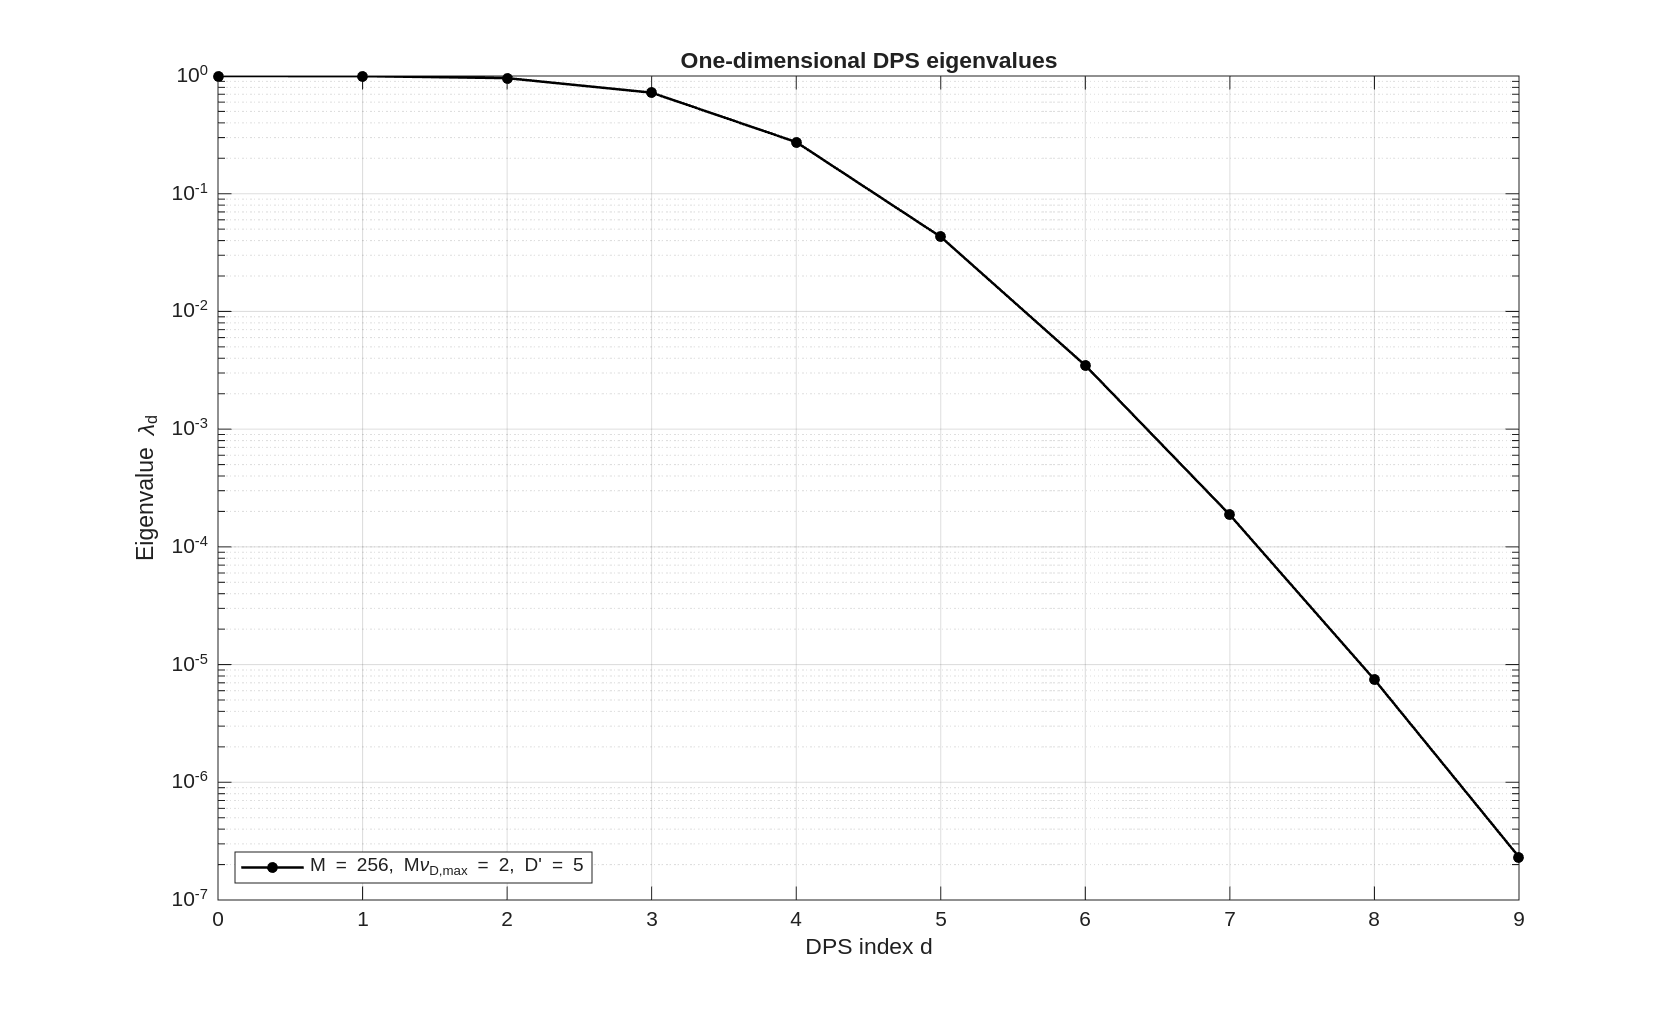
\includegraphics[width=0.9\textwidth]{results/figures/paper_figure4_dps_eigenvalues.png}
    \caption{Mười trị riêng đầu tiên của chuỗi DPS một chiều với \(N=256\) và \(N\nu_{D,\max}=2\)}
    \label{fig:ch2_paper_figure4_dps_eigenvalues}
\end{figure}

Hình~\ref{fig:ch2_paper_figure4_dps_eigenvalues} cho thấy các trị riêng đầu có giá trị lớn, sau đó giảm nhanh qua vùng chuyển tiếp quanh \(d=4\)--\(5\). Cụ thể, \(\lambda_0\approx0{,}99994\), trong khi \(\lambda_5\approx4{,}30\times10^{-2}\) và \(\lambda_9\approx2{,}32\times10^{-7}\). Do đó, các véc-tơ DPS có chỉ số lớn đóng góp ngày càng ít vào việc biểu diễn tín hiệu nằm trong băng Doppler mục tiêu. Đây là cơ sở để thay một véc-tơ kênh có \(256\) mẫu bằng một số lượng nhỏ hơn nhiều hệ số DPS; trong ví dụ của bài báo, khoảng năm chiều đầu tạo thành phần không gian con thiết yếu.

Tuy nhiên, \(D'=5\) chỉ mô tả vị trí chuyển tiếp của phổ trị riêng trong cấu hình cụ thể này, không phải số chiều cố định cho mọi kênh. Khi yêu cầu sai số nghiêm ngặt, có thể giữ thêm một số véc-tơ sau \(D'\). Ngược lại, nếu băng chuẩn hóa rộng hơn hoặc độ dài khối thay đổi, số chiều thiết yếu cũng thay đổi theo tích độ dài--băng thông. Vì vậy, kết luận cần rút ra từ hình là \(D\) có thể nhỏ hơn đáng kể \(N\) khi kênh bị giới hạn trong một miền Doppler hẹp, chứ không phải mọi kênh dài \(256\) mẫu đều luôn chỉ cần đúng năm véc-tơ DPS.

Nếu chọn \(D\) véc-tơ DPS đầu tiên và đặt:
\begin{equation}
\mathbf{V}
=
\begin{bmatrix}
\mathbf{v}_0 & \mathbf{v}_1 & \cdots & \mathbf{v}_{D-1}
\end{bmatrix},
\label{eq:ch2_dps_basis}
\end{equation}
thì \(\mathbf{V}\in\mathbb{C}^{N\times D}\) là ma trận cơ sở của một không gian con \(D\) chiều. Giữ nhiều véc-tơ hơn thường làm giảm phần năng lượng bị loại bỏ, nhưng đồng thời làm tăng số hệ số và chi phí tái tạo. Vì vậy, lựa chọn \(D\) thể hiện sự đánh đổi giữa độ phức tạp và sai số cắt không gian con.

\subsection{Biểu diễn không gian con DPS}
\label{subsec:ch2_dps_subspace}

Sau khi có ma trận cơ sở \(\mathbf{V}\), véc-tơ kênh được xấp xỉ dưới dạng tổ hợp tuyến tính của \(D\) cột trong ma trận này:
\begin{equation}
\hat{\mathbf{h}}^{D}=\mathbf{V}\boldsymbol{\alpha},
\label{eq:ch2_dps_reconstruction}
\end{equation}
trong đó dấu mũ trên \(\hat{\mathbf{h}}^{D}\) cho biết đây là véc-tơ tái tạo bằng \(D\) cơ sở, còn \(\boldsymbol{\alpha}\in\mathbb{C}^{D}\) chứa trọng số của từng cơ sở. Nếu \(\mathbf{V}\) trực chuẩn, hệ số chiếu chính xác của toàn bộ véc-tơ kênh được tính bằng:
\begin{equation}
\boldsymbol{\alpha}_{\mathrm{exact}}
= \mathbf{V}^{H}\mathbf{h}.
\label{eq:ch2_exact_projection}
\end{equation}
trong đó ký hiệu \((\cdot)^H\) là phép chuyển vị liên hợp. Công thức \eqref{eq:ch2_exact_projection} có ý nghĩa kiểm chứng rõ ràng: nếu tái tạo từ \(\boldsymbol{\alpha}_{\mathrm{exact}}\) cho sai số nhỏ, các \(D\) véc-tơ đã chọn giữ được phần quan trọng của khối kênh.

Có hai cách tương đương để thực hiện phép chiếu chính xác. Cách thứ nhất tạo toàn bộ \(\mathbf{h}\) bằng SoCE rồi áp dụng \eqref{eq:ch2_exact_projection}; cách này phù hợp để diễn giải nhưng vẫn phải tính đủ kênh tham chiếu. Cách thứ hai khai thác tính tuyến tính của phép chiếu: chiếu riêng véc-tơ hàm mũ của từng MPC lên \(\mathbf{V}\), nhân với \(\eta_p\), rồi cộng các hệ số. Mã mô phỏng dùng cách thứ hai và tiếp tục tách phép chiếu theo từng chiều. Phép chiếu vẫn là chính xác đối với cơ sở đã chọn, nhưng chi phí còn phụ thuộc vào tích giữa độ dài tín hiệu và số chiều cơ sở.

Để giảm tiếp chi phí tính các tích vô hướng này, bài báo Kaltenberger và cộng sự sử dụng công thức hàm sóng DPS nhằm xấp xỉ hệ số trực tiếp từ tần số của từng MPC \cite{Kaltenberger2007}. Trong đồ án, cách tính đó được gọi là DPS xấp xỉ. Như vậy, cần phân biệt sai số cắt do chỉ giữ \(D\) cơ sở với sai số bổ sung do dùng công thức xấp xỉ hệ số.

\subsection{So sánh cơ chế tính toán giữa SoCE và DPS}
\label{subsec:ch2_soce_dps_compare}

Sự khác nhau chính giữa SoCE và DPS nằm ở cách tổ chức phép tính. Với SoCE trực tiếp, giá trị kênh tại mỗi mẫu được tạo bằng cách cộng đóng góp của toàn bộ \(P\) MPC:
\begin{equation}
h_m
=\sum_{p=0}^{P-1}\eta_p e^{j2\pi\nu_p m}.
\label{eq:ch2_soce_samplewise}
\end{equation}
Cách tính này bám sát mô hình vật lý nhưng chi phí tăng theo cả số mẫu và số MPC. Ngược lại, với DPS, khối mẫu được biểu diễn thông qua các hệ số trong không gian con:
\begin{equation}
\hat{h}_m^{D}
= \sum_{d=0}^{D-1}\alpha_d v_d[m].
\label{eq:ch2_dps_samplewise}
\end{equation}
Khi \(D<N\), biểu diễn \eqref{eq:ch2_dps_samplewise} dùng ít hệ số hơn số mẫu ban đầu. Tuy nhiên, điều này chưa tự động bảo đảm tổng chi phí nhỏ hơn, vì vẫn phải tính hệ số và tái tạo \(N\) mẫu khi cần toàn bộ khối kênh. Lợi thế chỉ xuất hiện khi \(D\) đủ nhỏ và hai bước này được tổ chức hiệu quả.

Với tín hiệu giới hạn trong miền tần số chuẩn hóa \([-W,W]\) và chỉ xét trên \(N\) mẫu, lý thuyết DPS cho thấy số trị riêng lớn của bài toán \eqref{eq:ch2_dps_eigen} xấp xỉ bằng tích thời gian--băng thông \(2NW\) \cite{Slepian1978}. Do đó, số chiều DPS thiết yếu thường được chọn theo dạng:
\begin{equation}
D \approx 2NW + \Delta_D,
\label{eq:ch2_essential_dimension}
\end{equation}
trong đó \(\Delta_D\) là số chiều dự phòng được cộng thêm để giảm sai số cắt; giá trị cuối cùng của \(D\) phải là số nguyên. Khi \(W\) hẹp hơn đáng kể so với toàn miền tần số chuẩn hóa, \(2NW\) có thể nhỏ hơn nhiều so với \(N\). Khi đó, việc dùng các véc-tơ DPS đầu tiên có cơ sở từ cấu trúc giới hạn băng, thay vì chỉ là lựa chọn tùy ý. Trong mô phỏng của đồ án, số chiều dự phòng được chọn theo một quy tắc cố định và sẽ được nêu ở Chương 3.

Lập luận trên phù hợp với bài báo của Kaltenberger và cộng sự, trong đó kênh GCM sau rời rạc hóa được xem là tín hiệu giới hạn băng theo từng chiều và được chiếu lên không gian con DPS có số chiều hữu hạn \cite{Kaltenberger2007}. Như vậy, lợi thế của DPS không đến từ việc loại bỏ MPC khỏi mô hình, mà đến từ việc các tổ hợp SoCE có cùng miền giới hạn băng có thể được mô tả trong một không gian con chung. Nói cách khác, DPS chuyển bài toán từ tính từng tia truyền tại từng mẫu sang biểu diễn khối kênh bằng các hệ số không gian con.

Trong trường hợp nhiều chiều, khối mẫu được lưu dưới dạng tensor, tức mảng có nhiều hơn hai chiều. Giả sử tensor có kích thước \(N_1\times N_2\times\cdots\times N_L\), còn số véc-tơ DPS được giữ lại trên từng chiều là \(D_1,D_2,\ldots,D_L\). Khi đó, tổng số hệ số của biểu diễn tensor là:
\begin{equation}
D_{\mathrm{total}}=\prod_{\ell=1}^{L}D_\ell.
\label{eq:ch2_dps_total_dimension}
\end{equation}
Nếu chiều thứ \(\ell\) có nửa băng thông chuẩn hóa \(W_\ell\), lập luận thời gian--băng thông cho phép xấp xỉ:
\begin{equation}
D_{\mathrm{total}}
\approx
\prod_{\ell=1}^{L}\left(2N_\ell W_\ell+\Delta_{D_\ell}\right).
\label{eq:ch2_dps_total_dimension_approx}
\end{equation}
So sánh \eqref{eq:ch2_dps_total_dimension_approx} với tổng số mẫu \(\prod_{\ell=1}^{L}N_\ell\) cho thấy lợi thế về số chiều xuất hiện khi các miền băng \(W_\ell\) đủ hẹp để \(D_\ell<N_\ell\), đặc biệt khi điều kiện này đồng thời xảy ra trên nhiều chiều. Mức giảm thực tế còn phụ thuộc vào kích thước khối mẫu và sai số cắt không gian con được chấp nhận.

\subsection{Đối chứng triển khai cho biểu diễn DPS}
\label{subsec:ch2_alternative_baselines}

SoCE trực tiếp là tham chiếu tự nhiên vì bám sát các tham số vật lý của từng MPC. Tuy nhiên, nếu chỉ so sánh DPS với một cách cài đặt SoCE chưa tối ưu, phần giảm thời gian quan sát được có thể đến từ cách tính hàm mũ thay vì từ việc giảm số chiều. Vì vậy, SoCE cập nhật pha đệ quy được dùng như một đối chứng triển khai: phương pháp này giữ nguyên tập MPC và mô hình vật lý, nhưng thay cách tạo các thừa số pha. Đối chứng này giúp đánh giá liệu lợi thế của DPS còn được duy trì khi SoCE đã được tối ưu ở mức tạo pha.

\subsubsection{SoCE cập nhật pha đệ quy}
\label{subsubsec:ch2_recursive_soce}

Đặt \(z_p[m]=e^{j2\pi\nu_p m}\) và hệ số quay pha \(\rho_p=e^{j2\pi\nu_p}\). Các mẫu liên tiếp của MPC thứ \(p\) thỏa mãn:
\begin{equation}
z_p[0]=1,
\qquad
z_p[m+1]=\rho_p z_p[m].
\label{eq:ch2_recursive_phasor}
\end{equation}
Sau khi tính \(\rho_p\) một lần, các mẫu tiếp theo được tạo bằng phép nhân phức thay vì gọi lại hàm mũ. Giá trị kênh vẫn được cộng theo
\begin{equation}
h_m=\sum_{p=0}^{P-1}\eta_p z_p[m].
\label{eq:ch2_recursive_soce}
\end{equation}
Trong số học chính xác, \eqref{eq:ch2_recursive_soce} tương đương với SoCE trực tiếp trong \eqref{eq:ch2_1d_soce}; phương pháp không cắt bớt MPC và không lượng tử hóa tần số. Đối với lưới bốn chiều, quan hệ đệ quy có thể được áp dụng riêng cho các thừa số pha theo thời gian, tần số, anten phát và anten thu. Bậc độ phức tạp vẫn là \(\mathcal{O}(PN_{\mathrm{s}})\), nhưng số lần đánh giá hàm mũ được chuyển chủ yếu sang bước khởi tạo. Đổi lại, phép nhân lặp trong số học dấu phẩy động có thể tích lũy sai số biên độ và pha trên khối rất dài. Do đó, đây là đối chứng cần thiết để đánh giá liệu lợi thế của DPS còn được duy trì khi SoCE đã được tối ưu ở mức tạo pha.

\subsection{So sánh độ phức tạp và số phép tính}
\label{subsec:ch2_operation_count}

Phần trên so sánh số chiều biểu diễn. Để chuyển sang chi phí tính toán, cần tách ba nhóm phép toán của DPS: tính các hệ số một chiều, ghép chúng thành tensor hệ số và tái tạo khối mẫu. Trước hết, ký hiệu:
\begin{equation}
N_{\mathrm{s}}
=MQN_{\mathrm{Tx}}N_{\mathrm{Rx}}
\label{eq:ch2_total_samples}
\end{equation}
là tổng số mẫu của một khối kênh MIMO băng rộng. Với SoCE trực tiếp, mỗi mẫu cần cộng đóng góp của \(P\) MPC. Vì vậy, số hạng MPC--mẫu cần xử lý là:
\begin{equation}
N_{\mathrm{SoCE}}
=PN_{\mathrm{s}}
=PMQN_{\mathrm{Tx}}N_{\mathrm{Rx}}.
\label{eq:ch2_soce_operation_count}
\end{equation}
Nếu các hàm mũ một chiều đã được tạo trước, mỗi số hạng trong \eqref{eq:ch2_soce_operation_count} vẫn cần các phép nhân phức để ghép bốn chiều và cộng vào kênh tổng. Do đó, bậc độ phức tạp của SoCE trực tiếp vẫn là \(\mathcal{O}(PN_{\mathrm{s}})\).

Với biểu diễn DPS bốn chiều, ký hiệu \(D_t\), \(D_f\), \(D_{\mathrm{Tx}}\) và \(D_{\mathrm{Rx}}\) lần lượt là số véc-tơ DPS giữ lại trên các chiều thời gian, tần số, không gian phát và không gian thu. Số hệ số cần lưu trong tensor là \(D_{\mathrm{total}}=D_tD_fD_{\mathrm{Tx}}D_{\mathrm{Rx}}\). Nếu hệ số của từng MPC được tính bằng phép chiếu chính xác một chiều, chi phí tạo bốn véc-tơ hệ số một chiều có bậc:
\begin{equation}
C_{\gamma,\mathrm{exact}}
=
\mathcal{O}\!\left(
P(MD_t+QD_f+N_{\mathrm{Tx}}D_{\mathrm{Tx}}+N_{\mathrm{Rx}}D_{\mathrm{Rx}})
\right).
\label{eq:ch2_exact_gamma_complexity}
\end{equation}
Sau đó, việc cộng đóng góp của từng MPC vào tensor hệ số cần thêm:
\begin{equation}
C_{\alpha,\mathrm{4D}}
=
\mathcal{O}\!\left(PD_tD_fD_{\mathrm{Tx}}D_{\mathrm{Rx}}\right).
\label{eq:ch2_alpha_4d_complexity}
\end{equation}
Tiếp theo, tensor hệ số được nhân lần lượt với ma trận cơ sở trên từng chiều; thao tác trên một chiều của tensor thường được gọi là phép nhân theo mode. Chi phí tái tạo có bậc:
\begin{equation}
\begin{aligned}
C_{\mathrm{rec},\mathrm{4D}}
=\mathcal{O}\big(
&MD_tD_fD_{\mathrm{Tx}}D_{\mathrm{Rx}}
+MQD_fD_{\mathrm{Tx}}D_{\mathrm{Rx}}\\
&+MQN_{\mathrm{Tx}}D_{\mathrm{Tx}}D_{\mathrm{Rx}}
+MQN_{\mathrm{Tx}}N_{\mathrm{Rx}}D_{\mathrm{Rx}}
\big).
\end{aligned}
\label{eq:ch2_4d_reconstruction_complexity}
\end{equation}
Các biểu thức \eqref{eq:ch2_exact_gamma_complexity}--\eqref{eq:ch2_4d_reconstruction_complexity} cho thấy DPS tổ chức lại phép tính: phần phụ thuộc vào số MPC được chuyển chủ yếu sang việc tạo tensor hệ số có kích thước \(D_{\mathrm{total}}\), sau đó kênh được tái tạo từ tensor này. Khi các \(D\) đủ nhỏ so với số mẫu tương ứng, tổng số phép tính có khả năng giảm; ngược lại, nếu các \(D\) tiến gần kích thước khối, chi phí tái tạo có thể làm mất lợi thế.

Đối với nhánh DPS xấp xỉ 4D, hệ số một chiều được tính trực tiếp từ tần số chuẩn hóa của MPC bằng công thức hàm sóng DPS, thay vì chiếu chính xác lên toàn bộ véc-tơ hàm mũ. Nếu bỏ qua chi phí tiền xử lý cơ sở độ phân giải cao, phần hệ số một chiều có bậc:
\begin{equation}
C_{\gamma,\mathrm{approx}}
=
\mathcal{O}\!\left(P(D_t+D_f+D_{\mathrm{Tx}}+D_{\mathrm{Rx}})\right).
\label{eq:ch2_approx_gamma_complexity}
\end{equation}
Phương pháp kết hợp (hybrid) chỉ dùng DPS ở hai chiều thời gian và tần số, còn đáp ứng theo từng cặp anten được giữ trực tiếp. Khi đó tensor hệ số có kích thước \(D_tD_fN_{\mathrm{Tx}}N_{\mathrm{Rx}}\), và chi phí tái tạo chính là:
\begin{equation}
C_{\mathrm{rec},\mathrm{hybrid}}
=
\mathcal{O}\!\left(
MD_tD_fN_{\mathrm{Tx}}N_{\mathrm{Rx}}
+MQD_fN_{\mathrm{Tx}}N_{\mathrm{Rx}}
\right).
\label{eq:ch2_hybrid_reconstruction_complexity}
\end{equation}

Để đặt các biểu thức trên trong cùng một khung so sánh, Bảng~\ref{tab:ch2_complexity_comparison} tóm tắt bậc độ phức tạp và nguồn sai số của các phương pháp.

\begin{table}[H]
    \centering
    \small
    \caption{So sánh lý thuyết giữa SoCE và các nhánh DPS}
    \label{tab:ch2_complexity_comparison}
    \begin{tabularx}{\textwidth}{>{\raggedright\arraybackslash}p{0.17\textwidth} >{\raggedright\arraybackslash}p{0.25\textwidth} >{\raggedright\arraybackslash}p{0.24\textwidth} >{\raggedright\arraybackslash}X}
        \toprule
        Phương pháp & Phần phụ thuộc MPC hoặc hệ số & Tái tạo khối kênh & Đặc điểm sai số và điều kiện áp dụng \\
        \midrule
        SoCE trực tiếp
        & Không có bước hệ số riêng
        & \(\mathcal{O}(PN_{\mathrm{s}})\)
        & Tham chiếu theo mô hình MPC; chi phí tăng theo cả \(P\) và số mẫu. \\
        SoCE đệ quy
        & Khởi tạo các hệ số quay pha theo từng MPC và từng chiều
        & \(\mathcal{O}(PN_{\mathrm{s}})\)
        & Tương đương SoCE về mặt toán học; giảm số lần gọi hàm mũ nhưng có thể tích lũy sai số làm tròn. \\
        DPS chính xác 4D
        & \(C_{\gamma,\mathrm{exact}}+\mathcal{O}(PD_{\mathrm{total}})\)
        & \(C_{\mathrm{rec},\mathrm{4D}}\)
        & Hệ số chiếu chính xác trên cơ sở giữ lại; còn sai số cắt không gian con. \\
        DPS xấp xỉ 4D
        & \(\mathcal{O}(P\sum_iD_i)+\mathcal{O}(PD_{\mathrm{total}})\)
        & \(C_{\mathrm{rec},\mathrm{4D}}\)
        & Có sai số cắt và sai số xấp xỉ hệ số; cần bộ nhớ cho cơ sở độ phân giải cao. \\
        Hybrid DPS
        & Tạo hệ số DPS theo thời gian--tần số và giữ trực tiếp hai chiều không gian
        & \(C_{\mathrm{rec},\mathrm{hybrid}}\)
        & Tránh xấp xỉ DPS theo không gian; phù hợp khi số anten nhỏ so với số mẫu thời gian--tần số. \\
        \bottomrule
    \end{tabularx}
\end{table}

Bảng~\ref{tab:ch2_complexity_comparison} cho thấy SoCE đệ quy không thay đổi bậc \(\mathcal{O}(PN_{\mathrm{s}})\); lợi ích của nó nằm ở hằng số thực thi. DPS tổ chức lại phép tính thông qua không gian con, nên lợi thế của nó xuất hiện khi \(D_i\ll N_i\) trên các chiều có miền băng hẹp. Vì vậy, một đánh giá thực nghiệm công bằng phải dùng cùng tập MPC, cùng khối đầu ra và tính cả thời gian tiền xử lý, tạo hệ số lẫn tái tạo.

Bảng~\ref{tab:ch2_operation_estimate} minh họa các đại lượng trên với cấu hình hiện tại: \(M=256\), \(Q=64\), \(N_{\mathrm{Tx}}=N_{\mathrm{Rx}}=4\), \(P=80\), \(D_t=6\), \(D_f=9\) và \(D_{\mathrm{Tx}}=D_{\mathrm{Rx}}=4\). Các giá trị là ước lượng từ kích thước mảng và các biểu thức độ phức tạp, không phải số đếm chính xác mọi phép toán của MATLAB. Các số đo thời gian chạy được trình bày riêng ở Chương 4.

\begin{table}[H]
    \centering
    \small
    \caption{Ước lượng số phép xử lý chính với cấu hình mô phỏng hiện tại}
    \label{tab:ch2_operation_estimate}
    \begin{tabularx}{\textwidth}{l r >{\raggedright\arraybackslash}X}
        \toprule
        Đại lượng & Giá trị & Ý nghĩa \\
        \midrule
        \(N_{\mathrm{s}}=MQN_{\mathrm{Tx}}N_{\mathrm{Rx}}\) & \(262144\) & Số mẫu của một khối kênh 4D \\
        \(D_{\mathrm{total}}=D_tD_fD_{\mathrm{Tx}}D_{\mathrm{Rx}}\) & \(864\) & Số hệ số của biểu diễn DPS 4D \\
        \(N_{\mathrm{s}}/D_{\mathrm{total}}\) & \(\approx 303\) & Tỉ lệ giữa số mẫu kênh và số hệ số DPS 4D \\
        \(PN_{\mathrm{s}}\) & \(20971520\) & Số hạng MPC--mẫu trong SoCE trực tiếp \\
        \(4PN_{\mathrm{s}}\) & \(83886080\) & Ước lượng phép nhân phức để ghép bốn chiều nếu các hàm mũ một chiều đã có \\
        \(P(MD_t+QD_f+N_{\mathrm{Tx}}D_{\mathrm{Tx}}+N_{\mathrm{Rx}}D_{\mathrm{Rx}})\) & \(171520\) & Phép chiếu một chiều trong nhánh DPS chính xác \\
        \(PD_{\mathrm{total}}\) & \(69120\) & Cập nhật tensor hệ số DPS 4D theo từng MPC \\
        \(C_{\mathrm{rec},\mathrm{4D}}\) & \(4677632\) & Ước lượng phép nhân--cộng khi tái tạo DPS 4D \\
        \(C_{\mathrm{rec},\mathrm{hybrid}}\) & \(2580480\) & Ước lượng phép nhân--cộng khi tái tạo phương pháp hybrid \\
        \bottomrule
    \end{tabularx}
\end{table}

Từ Bảng~\ref{tab:ch2_operation_estimate}, số hệ số DPS 4D bằng \(864\), trong khi khối kênh chứa \(262144\) mẫu, tương ứng tỉ lệ xấp xỉ \(303\). Tỉ lệ này cho thấy khả năng nén về số hệ số, nhưng không đồng nghĩa thời gian chạy giảm đúng \(303\) lần vì vẫn có chi phí tạo cơ sở, tính hệ số và tái tạo. Trong cùng bảng, các ước lượng cho phép chiếu, cập nhật hệ số và tái tạo nhỏ hơn số hạng MPC--mẫu của SoCE trực tiếp trong cấu hình đang xét. Vì vậy, kết luận phù hợp là DPS có khả năng giảm độ phức tạp khi miền băng hẹp và \(D_{\mathrm{total}}\ll N_{\mathrm{s}}\), chứ không phải luôn có lợi trong mọi cấu hình.

\subsection{Ba mức tính hệ số trong đồ án}
\label{subsec:ch2_three_coefficients}

Để giữ thống nhất giữa lý thuyết và mô phỏng MATLAB, cần phân biệt ba nhánh theo cách tạo hệ số hoặc theo các chiều áp dụng DPS.

Thứ nhất, nhánh DPS chính xác tính tích vô hướng giữa véc-tơ hàm mũ của từng MPC và cơ sở DPS, sau đó ghép các hệ số một chiều thành tensor. Từ ``chính xác'' ở đây chỉ cách tính hệ số chiếu đối với cơ sở đã chọn; kênh tái tạo vẫn có thể có sai số vì cơ sở đã bị cắt còn \(D\) chiều. Nếu nhánh này có sai số nhỏ so với SoCE tham chiếu, số chiều DPS đang giữ là phù hợp với miền băng và khối mẫu đang xét.

Thứ hai, nhánh DPS xấp xỉ 4D thay các tích vô hướng chính xác bằng công thức hàm sóng DPS được đánh giá tại tần số chuẩn hóa của MPC. Công thức được áp dụng trên cả bốn chiều, nên sai số của nhánh này gồm cả sai số cắt không gian con và sai số xấp xỉ hệ số.

Thứ ba, phương pháp hybrid dùng hệ số DPS xấp xỉ cho hai chiều thời gian và tần số, trong khi phần không gian anten được tính bằng các hàm mũ trực tiếp. Với số anten nhỏ, số chiều không gian vốn đã thấp nên việc tiếp tục thay bằng cơ sở DPS có thể đem lại ít lợi ích hơn so với chi phí phát sinh. Nhánh hybrid vì vậy giữ khả năng giảm số chiều ở thời gian và tần số, đồng thời tránh xấp xỉ hệ số DPS trên hai chiều không gian.

\subsection{Đánh đổi khi sử dụng DPS}
\label{subsec:ch2_tradeoff}

DPS không làm cho mô phỏng kênh luôn đơn giản hơn trong mọi cấu hình. Lợi thế có khả năng xuất hiện khi miền tần số chuẩn hóa hẹp và số chiều thiết yếu nhỏ hơn đáng kể số mẫu ban đầu. Trong trường hợp đó, kênh được mô tả bằng ít hệ số hơn; với phép chiếu chính xác, sai số tái tạo chủ yếu đến từ phần năng lượng nằm ngoài không gian con đã chọn.

Ngược lại, nếu miền giới hạn băng rộng, tích \(2NW\) lớn hoặc số chiều dự phòng cao, \(D\) có thể tiến gần \(N\). Khi đó, lợi thế về số chiều giảm. Ngoài ra, cách tính hệ số xấp xỉ cần cơ sở trên lưới có độ phân giải cao để hạn chế sai số, làm phát sinh chi phí bộ nhớ và tiền xử lý. Vì vậy, việc sử dụng DPS phải được đánh giá đồng thời theo \(N\), \(W\), \(D\), số MPC, độ phân giải xấp xỉ và nhu cầu tái tạo toàn bộ khối kênh.

Trong phạm vi mô phỏng hiện tại, SoCE được dùng làm kênh tham chiếu; DPS chính xác dùng để đánh giá chất lượng không gian con; DPS xấp xỉ 4D và phương pháp hybrid dùng để khảo sát khả năng giảm độ phức tạp khi hệ số không được tính từ toàn bộ khối SoCE. Ngoài nhóm nhánh DPS này, SoCE đệ quy đóng vai trò đối chứng để kiểm tra ảnh hưởng của cách tạo pha.

\subsection{Kết luận chương}
\label{subsec:ch2_conclusion}

Chương này đã trả lời hai câu hỏi đầu chương. DPS giảm số chiều biểu diễn bằng cách dùng các véc-tơ cơ sở có mức tập trung năng lượng cao trong miền băng của kênh; số chiều thiết yếu được liên hệ với tích \(2NW\). So với việc tính từng MPC tại từng mẫu bằng SoCE, DPS tổ chức phép tính thành các bước tạo hệ số và tái tạo từ không gian con. SoCE đệ quy cho thấy việc tối ưu tạo pha có thể giảm hằng số thực thi nhưng không thay đổi bậc phụ thuộc \(PN_{\mathrm{s}}\). Vì vậy, lợi thế của DPS chỉ có khả năng xuất hiện khi số chiều giữ lại đủ nhỏ và chi phí tạo cơ sở, tính hệ số, tái tạo không làm mất phần tiết kiệm. Chương 3 tiếp tục cụ thể hóa các đại lượng này cho mô hình MIMO băng rộng bốn chiều và các nhánh mô phỏng MATLAB.

\cleardoublepage

    \chaptercustom{3}{MÔ HÌNH HỆ THỐNG VÀ TRIỂN KHAI MÔ PHỎNG}
\setcounter{section}{3}
\label{chap:system_simulation}

\subsection{Cấu hình kênh MIMO băng rộng}
\label{subsec:ch3_mimo_configuration}

Chương 2 đã phân tích cơ sở lý thuyết của biểu diễn DPS đối với tín hiệu giới hạn băng trên khối hữu hạn. Chương này chuyển phần lý thuyết đó thành một mô hình kênh và một quy trình mô phỏng cụ thể. Trình tự trình bày gồm bốn bước: mô tả ý nghĩa vật lý của kênh MIMO băng rộng; lấy mẫu kênh theo bốn chiều; xây dựng cơ sở DPS từ miền giới hạn băng; và triển khai các nhánh so sánh trong MATLAB. Nhờ đó, mỗi ký hiệu toán học đều có thể đối chiếu với một đại lượng vật lý hoặc một biến trong chương trình.

Xét hệ thống MIMO băng rộng gồm \(N_{\mathrm{Tx}}\) anten phát và \(N_{\mathrm{Rx}}\) anten thu. Mỗi cặp anten phát--thu tạo thành một kênh con; do đó, đáp ứng của toàn hệ thống phải mô tả đồng thời nhiều kênh con thay vì chỉ một tín hiệu vô tuyến. Các anten được giả thiết tạo thành mảng tuyến tính đều (Uniform Linear Array, ULA) với khoảng cách chuẩn hóa \(D_s/\lambda=0{,}5\), trong đó \(D_s\) là khoảng cách giữa hai phần tử anten liên tiếp và \(\lambda\) là bước sóng sóng mang.

Đáp ứng kênh được mô hình hóa theo GCM, trong đó tín hiệu từ máy phát đến máy thu qua nhiều đường truyền do phản xạ hoặc tán xạ. Mỗi đường được biểu diễn bằng một MPC. MPC thứ \(p\) có trọng số phức \(\eta_p\), dịch Doppler \(\omega_p\), trễ \(\tau_p\), góc khởi hành \(\phi_p\) và góc tới \(\psi_p\). Trọng số \(\eta_p\) chứa cả biên độ và pha ban đầu của đường truyền; bốn đại lượng còn lại quyết định sự thay đổi pha theo thời gian, tần số và vị trí anten.

Theo mô hình trong bài báo Kaltenberger và cộng sự, đáp ứng kênh phụ thuộc đồng thời vào thời gian \(t\), tần số khảo sát \(f\), vị trí anten phát \(x\) và vị trí anten thu \(y\) \cite{Kaltenberger2007}. Ở đây, \(f\) là vị trí tần số trong băng tín hiệu, không phải tần số sóng mang \(f_c\).

Hình~\ref{fig:ch3_gcm_mimo} minh họa cách GCM mô tả kênh MIMO thông qua các đường truyền trực tiếp hoặc phản xạ qua các vật tán xạ. Trong mỗi đường truyền, góc khởi hành tại phía phát và góc tới tại phía thu quyết định thành phần pha không gian của MPC tương ứng.

\begin{figure}[H]
    \centering
    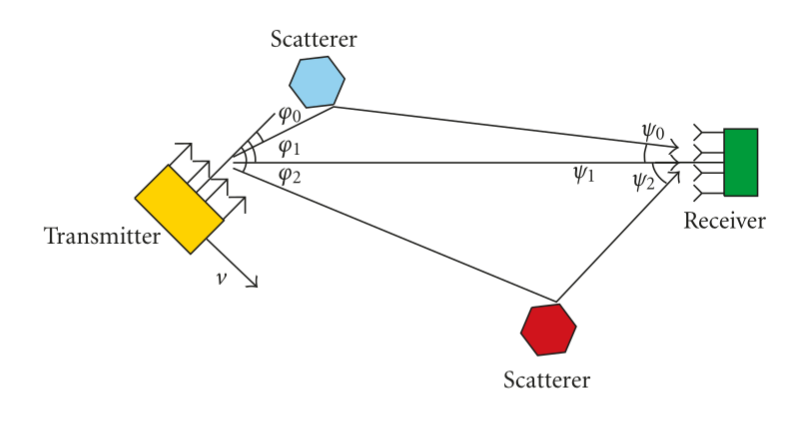
\includegraphics[width=0.82\textwidth]{results/figures/gcm_MIMO.png}
    \caption{Minh họa mô hình kênh MIMO dựa trên hình học với các thành phần đa đường}
    \label{fig:ch3_gcm_mimo}
\end{figure}

Trong mô hình toán học, mỗi đường truyền trong Hình~\ref{fig:ch3_gcm_mimo} được biểu diễn bằng một MPC có trọng số phức, dịch Doppler, trễ truyền lan và hai góc không gian. Tổng đóng góp của các MPC tạo thành đáp ứng kênh liên tục:
\begin{equation}
h(t,f,x,y)
=
\sum_{p=0}^{P-1}
\eta_p
e^{j2\pi \omega_p t}
e^{-j2\pi \tau_p f}
e^{j\frac{2\pi}{\lambda}\sin(\phi_p)x}
e^{-j\frac{2\pi}{\lambda}\sin(\psi_p)y}.
\label{eq:ch3_continuous_gcm}
\end{equation}
Dấu pha trong \eqref{eq:ch3_continuous_gcm} thể hiện bốn cơ chế vật lý: Doppler theo thời gian, trễ theo tần số, pha không gian ở phía phát và pha không gian ở phía thu. Giá trị \(h(t,f,x,y)\) là một số phức biểu diễn hệ số kênh tại đúng thời điểm, tần số và cặp vị trí anten đang xét. Quy ước dấu này được giữ nhất quán trong mô hình rời rạc và trong hàm MATLAB \texttt{compute\_mimo\_soce}.

\subsection{Rời rạc hóa bốn chiều}
\label{subsec:ch3_discretization}

Để tính kênh trên máy tính, bốn biến liên tục được thay bằng các điểm lấy mẫu
\(t=mT_s\), \(f=qF_s\), \(x=sD_s\) và \(y=rD_s\). Chỉ số thời gian là \(m=0,\ldots,M-1\), chỉ số tần số là \(q=0,\ldots,Q-1\), chỉ số anten phát là \(s=0,\ldots,N_{\mathrm{Tx}}-1\), và chỉ số anten thu là \(r=0,\ldots,N_{\mathrm{Rx}}-1\). Vì vậy, một phần tử \(h_{m,q,s,r}\) là hệ số kênh giữa anten phát \(s\) và anten thu \(r\), tại mẫu thời gian \(m\) và điểm tần số \(q\).

Để số mũ phức chỉ còn phụ thuộc vào các chỉ số nguyên, các tham số vật lý được đổi thành tần số chuẩn hóa:
\begin{equation}
\nu_p = \omega_p T_s,
\quad
\theta_p = \tau_p F_s,
\quad
\zeta_p = \sin(\phi_p)\frac{D_s}{\lambda},
\quad
\xi_p = \sin(\psi_p)\frac{D_s}{\lambda},
\label{eq:ch3_normalized_variables}
\end{equation}
trong đó \(T_s\) là chu kỳ lấy mẫu theo thời gian và \(F_s\) là khoảng cách giữa hai điểm tần số liên tiếp trong mô phỏng. Các đại lượng \(\nu_p,\theta_p,\zeta_p,\xi_p\) không có đơn vị và biểu thị số chu kỳ pha trên một bước chỉ số ở từng chiều.

Thay \eqref{eq:ch3_normalized_variables} vào \eqref{eq:ch3_continuous_gcm}, đáp ứng kênh rời rạc bốn chiều có dạng:
\begin{equation}
h_{m,q,s,r}
=
\sum_{p=0}^{P-1}
\eta_p
e^{j2\pi(\nu_p m-\theta_p q+\zeta_p s-\xi_p r)}.
\label{eq:ch3_discrete_soce}
\end{equation}
Phương trình \eqref{eq:ch3_discrete_soce} cho thấy tại mỗi bộ chỉ số \((m,q,s,r)\), chương trình phải tính và cộng đóng góp của toàn bộ \(P\) MPC. Đây là SoCE tham chiếu trong mô phỏng. Trong MATLAB, tất cả các giá trị \(h_{m,q,s,r}\) được xếp vào mảng bốn chiều, còn gọi là tensor, \texttt{H\_soce} có kích thước \(M\times Q\times N_{\mathrm{Tx}}\times N_{\mathrm{Rx}}\).

Các tham số MPC trong mô phỏng hiện tại được sinh ngẫu nhiên trong miền giới hạn băng đã định trước. Trọng số \(\eta_p\) được sinh theo phân bố Gauss phức tròn với chuẩn hóa công suất trung bình, còn các tần số chuẩn hóa \(\nu_p,\theta_p,\zeta_p,\xi_p\) được lấy đều trong các khoảng vật lý tương ứng. Các giả thiết này dùng để kiểm tra biểu diễn DPS và không nhằm tái tạo đầy đủ một kịch bản kênh chuẩn cụ thể.

\subsection{Miền giới hạn băng}
\label{subsec:ch3_band_region}

Mặc dù khối kênh có nhiều phần tử, các hàm mũ trong \eqref{eq:ch3_discrete_soce} không thể có tần số tùy ý. Vận tốc cực đại giới hạn Doppler, độ trễ cực đại giới hạn biến thiên theo tần số, còn khoảng góc giới hạn biến thiên theo vị trí anten. Vì vậy, các tần số chuẩn hóa chỉ nằm trong miền:
\begin{equation}
\mathcal{W}
=
\mathcal{W}_t
\times
\mathcal{W}_f
\times
\mathcal{W}_{\mathrm{Tx}}
\times
\mathcal{W}_{\mathrm{Rx}}.
\label{eq:ch3_band_region}
\end{equation}
Trong script MATLAB, các miền thành phần được xác định bởi:
\begin{equation}
\mathcal{W}_t=[-\nu_{\mathrm{D,max}},\nu_{\mathrm{D,max}}],
\quad
\mathcal{W}_f=[-\theta_{\max},0],
\label{eq:ch3_time_frequency_bands}
\end{equation}
và:
\begin{equation}
\mathcal{W}_{\mathrm{Tx}}=[\zeta_{\min},\zeta_{\max}],
\quad
\mathcal{W}_{\mathrm{Rx}}=[-\xi_{\max},-\xi_{\min}].
\label{eq:ch3_spatial_bands}
\end{equation}
Trong đó:
\begin{equation}
\nu_{\mathrm{D,max}}
=
\frac{v_{\max} f_c T_s}{c},
\quad
\theta_{\max}=\tau_{\max}F_s.
\label{eq:ch3_doppler_delay_bounds}
\end{equation}
Các giới hạn không gian được tính từ khoảng góc tới và góc khởi hành:
\begin{equation}
\zeta_{\min,\max}=\sin(\phi_{\min,\max})\frac{D_s}{\lambda},
\quad
\xi_{\min,\max}=\sin(\psi_{\min,\max})\frac{D_s}{\lambda}.
\label{eq:ch3_spatial_bounds}
\end{equation}

Để tạo cơ sở DPS có thể dịch tâm tần số, mỗi chiều được mô tả bằng tâm băng \(W_0\) và nửa băng thông \(W_{\max}\). Cách ánh xạ trong MATLAB là:
\begin{equation}
\begin{aligned}
&\text{thời gian:}      && W_0=0,\quad W_{\max}=\nu_{\mathrm{D,max}},\\
&\text{tần số:}         && W_0=-\theta_{\max}/2,\quad W_{\max}=\theta_{\max}/2,\\
&\text{không gian phát:}&& W_0=(\zeta_{\min}+\zeta_{\max})/2,\quad
W_{\max}=(\zeta_{\max}-\zeta_{\min})/2,\\
&\text{không gian thu:} && W_0=-(\xi_{\min}+\xi_{\max})/2,\quad
W_{\max}=(\xi_{\max}-\xi_{\min})/2.
\end{aligned}
\label{eq:ch3_dps_band_mapping}
\end{equation}
Các dấu âm ở chiều tần số và chiều thu xuất phát từ dấu pha \(-\theta_p q\) và \(-\xi_p r\) trong \eqref{eq:ch3_discrete_soce}. Việc xác định đúng tâm băng và nửa băng thông là bước nối giữa mô hình vật lý với cơ sở DPS: cơ sở chỉ biểu diễn tốt kênh khi miền băng dùng để tạo cơ sở bao phủ các tần số của MPC.

\subsection{Cơ sở DPS đa chiều}
\label{subsec:ch3_multidim_dps}

Với miền giới hạn băng dạng tích Descartes trong \eqref{eq:ch3_band_region}, mỗi chiều có thể dùng một cơ sở DPS riêng. Gọi \(\mathbf{V}_t\), \(\mathbf{V}_f\), \(\mathbf{V}_{\mathrm{Tx}}\) và \(\mathbf{V}_{\mathrm{Rx}}\) lần lượt là các ma trận cơ sở DPS theo thời gian, tần số, anten phát và anten thu. Mỗi cột của một ma trận là một vector cơ sở; chẳng hạn, \(v^{(t)}_{d_t}[m]\) là giá trị của vector DPS thứ \(d_t\) tại mẫu thời gian \(m\).

Ý tưởng tái tạo là thay tổng theo các MPC trong \eqref{eq:ch3_discrete_soce} bằng tổng theo một số hữu hạn các hàm cơ sở. Hệ số \(\alpha_{d_t,d_f,d_{\mathrm{Tx}},d_{\mathrm{Rx}}}\) cho biết mức đóng góp của một tổ hợp gồm bốn vector cơ sở. Khi đó, xấp xỉ DPS bốn chiều có thể viết:
\begin{equation}
\hat{h}_{m,q,s,r}
=
\sum_{d_t=0}^{D_t-1}
\sum_{d_f=0}^{D_f-1}
\sum_{d_{\mathrm{Tx}}=0}^{D_{\mathrm{Tx}}-1}
\sum_{d_{\mathrm{Rx}}=0}^{D_{\mathrm{Rx}}-1}
\alpha_{d_t,d_f,d_{\mathrm{Tx}},d_{\mathrm{Rx}}}
v^{(t)}_{d_t}[m]
v^{(f)}_{d_f}[q]
v^{(\mathrm{Tx})}_{d_{\mathrm{Tx}}}[s]
v^{(\mathrm{Rx})}_{d_{\mathrm{Rx}}}[r].
\label{eq:ch3_4d_dps_reconstruction}
\end{equation}
Số hệ số của biểu diễn này là:
\begin{equation}
D_{\mathrm{total}}
=D_tD_fD_{\mathrm{Tx}}D_{\mathrm{Rx}}.
\label{eq:ch3_total_dps_dimension}
\end{equation}

Trong script, số vector DPS của từng chiều được chọn theo số chiều thiết yếu cộng thêm một số vector dự phòng:
\begin{equation}
\begin{aligned}
D_t  &= \left\lceil 2\nu_{\mathrm{D,max}}M \right\rceil + 1 + G,\\
D_f  &= \left\lceil \theta_{\max}Q \right\rceil + 1 + G,\\
D_{\mathrm{Tx}} &= \left\lceil (\zeta_{\max}-\zeta_{\min})N_{\mathrm{Tx}} \right\rceil + 1 + G,\\
D_{\mathrm{Rx}} &= \left\lceil (\xi_{\max}-\xi_{\min})N_{\mathrm{Rx}} \right\rceil + 1 + G.
\end{aligned}
\label{eq:ch3_dps_dimension_rule}
\end{equation}
Trong mô phỏng hiện tại, \(G=4\). Số hạng dự phòng này giữ thêm các vector ở rìa không gian con nhằm giảm sai số cắt. Các giá trị \(D_t,D_f,D_{\mathrm{Tx}},D_{\mathrm{Rx}}\) sau đó được chặn trên bởi số mẫu tương ứng của từng chiều, vì một chiều có \(N\) mẫu không thể có hơn \(N\) vector cơ sở độc lập. Quy tắc trên là giả thiết thiết kế của mô phỏng hiện tại, chưa phải thủ tục tự động chọn số chiều từ một ngưỡng sai số cho trước.

\subsection{Các nhánh mô phỏng MATLAB}
\label{subsec:ch3_simulation_branches}

Phiên bản mô phỏng xấp xỉ triển khai bốn nhánh chính trên cùng một tập MPC. Nhánh thứ nhất là SoCE tham chiếu, trong đó chương trình tính trực tiếp \eqref{eq:ch3_discrete_soce}. Ba nhánh còn lại không thay đổi kịch bản truyền sóng mà chỉ thay đổi cách biểu diễn và tái tạo cùng một kênh. Vì vậy, sai khác giữa chúng với SoCE phản ánh sai số của biểu diễn DPS trong cấu hình đang xét.

Nhánh thứ hai là DPS chính xác. Với mỗi MPC, script tạo các vector hàm mũ theo bốn chiều và chiếu chính xác lên từng cơ sở DPS:
\begin{equation}
\begin{aligned}
\boldsymbol{\gamma}^{(t)}_p
&=\mathbf{V}_t^{H}\mathbf{e}^{(t)}(\nu_p),&
\boldsymbol{\gamma}^{(f)}_p
&=\mathbf{V}_f^{H}\mathbf{e}^{(f)}(-\theta_p),\\
\boldsymbol{\gamma}^{(\mathrm{Tx})}_p
&=\mathbf{V}_{\mathrm{Tx}}^{H}\mathbf{e}^{(\mathrm{Tx})}(\zeta_p),&
\boldsymbol{\gamma}^{(\mathrm{Rx})}_p
&=\mathbf{V}_{\mathrm{Rx}}^{H}\mathbf{e}^{(\mathrm{Rx})}(-\xi_p).
\end{aligned}
\label{eq:ch3_exact_projection_coefficients}
\end{equation}
Tensor hệ số của toàn bộ kênh được tạo bằng tổng các tích ngoài:
\begin{equation}
\boldsymbol{\alpha}_{\mathrm{exact}}
=
\sum_{p=0}^{P-1}
\eta_p\,
\boldsymbol{\gamma}^{(t)}_p
\circ
\boldsymbol{\gamma}^{(f)}_p
\circ
\boldsymbol{\gamma}^{(\mathrm{Tx})}_p
\circ
\boldsymbol{\gamma}^{(\mathrm{Rx})}_p.
\label{eq:ch3_exact_alpha}
\end{equation}
Ký hiệu \(\circ\) trong \eqref{eq:ch3_exact_alpha} là tích ngoài: bốn vector hệ số một chiều được ghép thành một tensor hệ số bốn chiều. Nhánh này dùng để đánh giá chất lượng của không gian con DPS đã chọn. Tên gọi ``DPS chính xác'' chỉ có nghĩa các hệ số chiếu được tính bằng tích vô hướng chính xác; kênh tái tạo vẫn có thể sai khác với SoCE do chỉ giữ một số hữu hạn vector DPS.

Nhánh thứ ba là DPS xấp xỉ 4D. Thay vì tạo toàn bộ vector hàm mũ rồi tính tích vô hướng như \eqref{eq:ch3_exact_projection_coefficients}, chương trình dùng hàm \texttt{approximate\_gamma\_1d(...)} để ước lượng trực tiếp hệ số một chiều từ vị trí tần số chuẩn hóa của MPC trên một cơ sở DPS có độ phân giải cao. Các hệ số này sau đó được ghép bằng tích ngoài giống \eqref{eq:ch3_exact_alpha}. Đây là nhánh kiểm tra việc áp dụng công thức xấp xỉ hàm sóng DPS cho cả bốn chiều.

Nhánh thứ tư là phương pháp hybrid. Nhánh này dùng DPS xấp xỉ cho hai chiều thời gian và tần số, nhưng giữ phần không gian anten dưới dạng hàm mũ trực tiếp:
\begin{equation}
\boldsymbol{\alpha}_{\mathrm{hybrid}}
=
\sum_{p=0}^{P-1}
\eta_p\,
\boldsymbol{\gamma}^{(t)}_p
\circ
\boldsymbol{\gamma}^{(f)}_p
\circ
\mathbf{e}^{(\mathrm{Tx})}(\zeta_p)
\circ
\mathbf{e}^{(\mathrm{Rx})}(-\xi_p).
\label{eq:ch3_hybrid_alpha}
\end{equation}
Trong MATLAB, nhánh này tương ứng với \texttt{build\_alpha\_approx\_hybrid(...)} và \texttt{reconstruct\_hybrid(...)}. Cách triển khai này phù hợp với định hướng thực tế của bài báo: khi số anten không lớn, lợi ích của DPS ở chiều không gian có thể hạn chế, trong khi DPS theo thời gian và tần số vẫn khai thác được cấu trúc giới hạn băng của kênh \cite{Kaltenberger2007}.

\subsection{Tham số và ánh xạ biến MATLAB}
\label{subsec:ch3_matlab_mapping}

Bảng~\ref{tab:ch3_simulation_parameters} tóm tắt các tham số chính đang dùng trong script mô phỏng. Đây là các tham số cấu hình, không phải kết quả đánh giá hiệu năng.

\begin{table}[H]
    \centering
    \small
    \caption{Tham số mô phỏng chính trong script MATLAB}
    \label{tab:ch3_simulation_parameters}
    \begin{tabularx}{\textwidth}{l l X}
        \toprule
        Ký hiệu & Biến MATLAB & Giá trị trong mô phỏng hiện tại \\
        \midrule
        \(f_c\) & \texttt{fc} & \(2\,\mathrm{GHz}\) \\
        \(v_{\max}\) & \texttt{vmax} & \(100/3{,}6\,\mathrm{m/s}\) \\
        \(T_s\) & \texttt{Ts} & \(1/3{,}84\,\mathrm{MHz}\) \\
        \(F_s\) & \texttt{Fbin} & \(15\,\mathrm{kHz}\) \\
        \(\tau_{\max}\) & \texttt{tau\_max} & \(3{,}7\,\mu\mathrm{s}\) \\
        \(D_s/\lambda\) & \texttt{d\_over\_lambda} & \(0{,}5\) \\
        \([\phi_{\min},\phi_{\max}]\) & \texttt{phi\_min}, \texttt{phi\_max} & \([-5^\circ,5^\circ]\) \\
        \([\psi_{\min},\psi_{\max}]\) & \texttt{psi\_min}, \texttt{psi\_max} & \([-5^\circ,5^\circ]\) \\
        \(M,Q\) & \texttt{M}, \texttt{Q} & \(256,64\) \\
        \(N_{\mathrm{Tx}},N_{\mathrm{Rx}}\) & \texttt{N\_Tx}, \texttt{N\_Rx} & \(4,4\) \\
        \(P\) & \texttt{P} & \(80\) \\
        \bottomrule
    \end{tabularx}
\end{table}

Bảng~\ref{tab:ch3_variable_mapping} trình bày ánh xạ giữa ký hiệu trong chương và biến MATLAB. Việc thống nhất ánh xạ này giúp đảm bảo các phương trình trong đồ án và mã mô phỏng sử dụng cùng quy ước dấu pha.

\begin{table}[H]
    \centering
    \small
    \caption{Ánh xạ ký hiệu mô hình với biến MATLAB}
    \label{tab:ch3_variable_mapping}
    \begin{tabularx}{\textwidth}{l l X}
        \toprule
        Ký hiệu & Biến MATLAB & Ý nghĩa \\
        \midrule
        \(h_{m,q,s,r}\) & \texttt{H\_soce} & Kênh SoCE tham chiếu \\
        \(\hat{h}_{m,q,s,r}\) & \texttt{H\_exact}, \texttt{H\_approx\_4d}, \texttt{H\_hybrid} & Kênh tái tạo từ các nhánh DPS \\
        \(\eta_p\) & \texttt{eta(p)} & Trọng số phức của MPC thứ \(p\) \\
        \(\nu_p\) & \texttt{nu(p)} & Dịch Doppler chuẩn hóa \\
        \(\theta_p\) & \texttt{theta(p)} & Trễ chuẩn hóa theo tần số \\
        \(\zeta_p\) & \texttt{zeta(p)} & Tần số không gian phía phát \\
        \(\xi_p\) & \texttt{xi(p)} & Tần số không gian phía thu \\
        \(\mathbf{V}_t,\mathbf{V}_f\) & \texttt{dim\_t.V}, \texttt{dim\_f.V} & Cơ sở DPS theo thời gian và tần số \\
        \(\mathbf{V}_{\mathrm{Tx}},\mathbf{V}_{\mathrm{Rx}}\) & \texttt{dim\_tx.V}, \texttt{dim\_rx.V} & Cơ sở DPS theo không gian phát và thu \\
        \(\boldsymbol{\alpha}_{\mathrm{exact}}\) & \texttt{alpha\_exact} & Hệ số DPS chiếu chính xác \\
        \(\boldsymbol{\alpha}_{\mathrm{approx}}\) & \texttt{alpha\_approx\_4d} & Hệ số DPS xấp xỉ 4D \\
        \(\boldsymbol{\alpha}_{\mathrm{hybrid}}\) & \texttt{alpha\_hybrid} & Hệ số phương pháp hybrid \\
        \bottomrule
    \end{tabularx}
\end{table}

\subsection{Quy trình mô phỏng}
\label{subsec:ch3_simulation_flow}

Quy trình mô phỏng trong MATLAB gồm các bước chính sau. Đầu tiên, chương trình thiết lập seed bằng \texttt{rng(1)} để bảo đảm khả năng tái lập. Tiếp theo, chương trình thiết lập tham số vật lý, sinh \(P\) MPC trong miền giới hạn băng và tạo các cơ sở DPS một chiều. Sau đó, kênh SoCE tham chiếu được tính theo \eqref{eq:ch3_discrete_soce}.

Hình~\ref{fig:ch3_simulation_flowchart} tóm tắt luồng xử lý chính của mô phỏng. Sơ đồ cho thấy SoCE được dùng làm nhánh tham chiếu, trong khi ba nhánh DPS được tính song song về mặt thuật toán trước khi so sánh sai số và thời gian chạy.

\begin{figure}[H]
    \centering
    \begin{tikzpicture}[
        block/.style={draw, rounded corners=2pt, align=center, text width=3.4cm, minimum height=0.95cm, font=\small},
        branch/.style={draw, rounded corners=2pt, align=center, text width=3.1cm, minimum height=1.1cm, font=\scriptsize},
        arrow/.style={->, thick}
    ]
        \node[block] (init) at (0,0) {Thiết lập seed và tham số mô phỏng};
        \node[block] (mpc) at (0,-1.55) {Sinh MPC trong miền giới hạn băng};
        \node[block] (basis) at (0,-3.10) {Tạo cơ sở DPS một chiều};
        \node[block] (soce) at (0,-4.65) {Tính kênh SoCE tham chiếu};

        \node[branch] (exact) at (-4.1,-6.35) {DPS chính xác\\Tính \(\boldsymbol{\alpha}_{\mathrm{exact}}\)};
        \node[branch] (approx) at (0,-6.35) {DPS xấp xỉ 4D\\Tính \(\boldsymbol{\alpha}_{\mathrm{approx}}\)};
        \node[branch] (hybrid) at (4.1,-6.35) {Phương pháp hybrid\\Tính \(\boldsymbol{\alpha}_{\mathrm{hybrid}}\)};

        \node[branch] (rexact) at (-4.1,-8.10) {Tái tạo\\\(\hat{H}_{\mathrm{exact}}\)};
        \node[branch] (rapprox) at (0,-8.10) {Tái tạo\\\(\hat{H}_{\mathrm{approx}}\)};
        \node[branch] (rhybrid) at (4.1,-8.10) {Tái tạo\\\(\hat{H}_{\mathrm{hybrid}}\)};

        \node[block, text width=4.2cm] (metrics) at (0,-9.95) {Tính MSE, NMSE, sai số cực đại và thời gian chạy};
        \node[block, text width=4.2cm] (outputs) at (0,-12.00) {Tạo hình và bảng phục vụ phân tích kết quả};

        \draw[arrow] (init) -- (mpc);
        \draw[arrow] (mpc) -- (basis);
        \draw[arrow] (basis) -- (soce);
        \draw[arrow] (soce) -- (exact);
        \draw[arrow] (soce) -- (approx);
        \draw[arrow] (soce) -- (hybrid);
        \draw[arrow] (exact) -- (rexact);
        \draw[arrow] (approx) -- (rapprox);
        \draw[arrow] (hybrid) -- (rhybrid);
        \draw[arrow] (rexact) -- (metrics);
        \draw[arrow] (rapprox) -- (metrics);
        \draw[arrow] (rhybrid) -- (metrics);
        \draw[arrow] (soce.east) -- ++(6.0,0) |- (metrics.east);
        \draw[arrow] (metrics) -- (outputs);
    \end{tikzpicture}
    \caption{Quy trình mô phỏng và đánh giá các nhánh biểu diễn kênh}
    \label{fig:ch3_simulation_flowchart}
\end{figure}

Sau khi có kênh tham chiếu, chương trình lần lượt tính hệ số cho ba nhánh DPS: chiếu chính xác, xấp xỉ 4D và phương pháp hybrid. Các tensor hệ số được tái tạo bằng phép nhân tensor theo từng mode thông qua hàm \texttt{mode\_product(...)}. Cuối cùng, chương trình tính các đại lượng sai số và thời gian chạy để phục vụ phần đánh giá ở Chương 4.

\subsection{Kết luận chương}
\label{subsec:ch3_conclusion}

Chương này đã trình bày mô hình GCM MIMO băng rộng, quá trình rời rạc hóa bốn chiều và cách triển khai các nhánh mô phỏng trong MATLAB. SoCE được dùng làm kênh tham chiếu; DPS chính xác dùng để kiểm tra không gian con; DPS xấp xỉ 4D kiểm tra công thức hệ số dựa trên hàm sóng DPS; và phương pháp hybrid kết hợp DPS theo thời gian--tần số với hàm mũ không gian trực tiếp. Cấu trúc này tạo cơ sở cho Chương 4 đánh giá sai số và thời gian tính toán của các nhánh mô phỏng.

\cleardoublepage

    \chaptercustom{4}{KẾT QUẢ MÔ PHỎNG VÀ THẢO LUẬN}
\setcounter{section}{4}
\label{chap:simulation_results}

\subsection{Nguồn dữ liệu và phạm vi đánh giá}
\label{subsec:ch4_data_scope}

Chương này đánh giá kết quả của quy trình mô phỏng đã trình bày ở Chương 3. Phần trình bày lần lượt trả lời ba câu hỏi: kênh tái tạo có giữ được dạng biến thiên của kênh SoCE hay không; sai số giữa các nhánh khác nhau như thế nào; và chi phí thời gian quan sát được trong lần chạy hiện tại là bao nhiêu. Các nhận xét định lượng chỉ dựa trên các hình và bảng kết quả đã được kiểm chứng.

Trong mô phỏng này, SoCE được dùng làm kênh tham chiếu vì nó tính trực tiếp đóng góp của từng MPC tại từng mẫu. Ba nhánh được so sánh với tham chiếu gồm DPS chính xác, DPS xấp xỉ 4D và phương pháp hybrid. Vì cả bốn nhánh dùng cùng một tập MPC, sai khác ở đầu ra xuất phát từ cách tính hệ số và tái tạo kênh, không phải từ một kịch bản truyền sóng khác. Việc đánh giá bắt đầu bằng quan sát định tính trên đáp ứng kênh, sau đó mới dùng chỉ tiêu sai số để định lượng mức sai khác.

Bảng~\ref{tab:ch4_simulation_config} tóm tắt cấu hình mô phỏng dùng cho phần đánh giá. Trong đó, \(M,Q\) xác định số mẫu thời gian và tần số; \(N_{\mathrm{Tx}},N_{\mathrm{Rx}}\) xác định kích thước mảng anten; \(P\) là số MPC; còn \(D_t,D_f,D_{\mathrm{Tx}},D_{\mathrm{Rx}}\) là số véc-tơ DPS được giữ lại ở bốn chiều. Các hệ số \(r\) biểu thị độ phân giải của cơ sở dùng khi xấp xỉ hệ số DPS, không phải số mẫu của khối kênh.

\begin{table}[H]
    \centering
    \small
    \caption{Cấu hình mô phỏng dùng cho kết quả Chương 4}
    \label{tab:ch4_simulation_config}
    \begin{tabular}{ll}
        \toprule
        Tham số & Giá trị \\
        \midrule
        \(M,Q,N_{\mathrm{Tx}},N_{\mathrm{Rx}}\) & \(256,64,4,4\) \\
        \(P\) & \(80\) MPC \\
        \(D_t,D_f,D_{\mathrm{Tx}},D_{\mathrm{Rx}}\) & \(6,9,4,4\) \\
        \(D_{\mathrm{total}}\) & \(864\) \\
        \(r_t,r_f,r_{\mathrm{Tx}},r_{\mathrm{Rx}}\) & \(2,512,512,512\) \\
        \(\nu_{\mathrm{D,max}}\) & \(4{,}8225\times10^{-5}\) \\
        \(\theta_{\max}\) & \(5{,}55\times10^{-2}\) \\
        \bottomrule
    \end{tabular}
\end{table}

\subsection{So sánh đáp ứng kênh}
\label{subsec:ch4_channel_response}

Trước hết, cần kiểm tra liệu phương pháp tái tạo có giữ được cấu trúc chung của đáp ứng kênh hay không. Hình~\ref{fig:mimo_dps_kaltenberger_approx_tx1_rx1} minh họa biên độ đáp ứng của cặp anten phát--thu thứ nhất. Trục \(m\) biểu diễn chỉ số mẫu thời gian, trục \(q\) biểu diễn chỉ số điểm tần số, còn màu sắc biểu diễn độ lớn của hệ số kênh phức. Bốn ô lần lượt thể hiện SoCE tham chiếu, DPS chính xác, phương pháp hybrid và sai số tuyệt đối giữa SoCE với hybrid.

\begin{figure}[H]
    \centering
    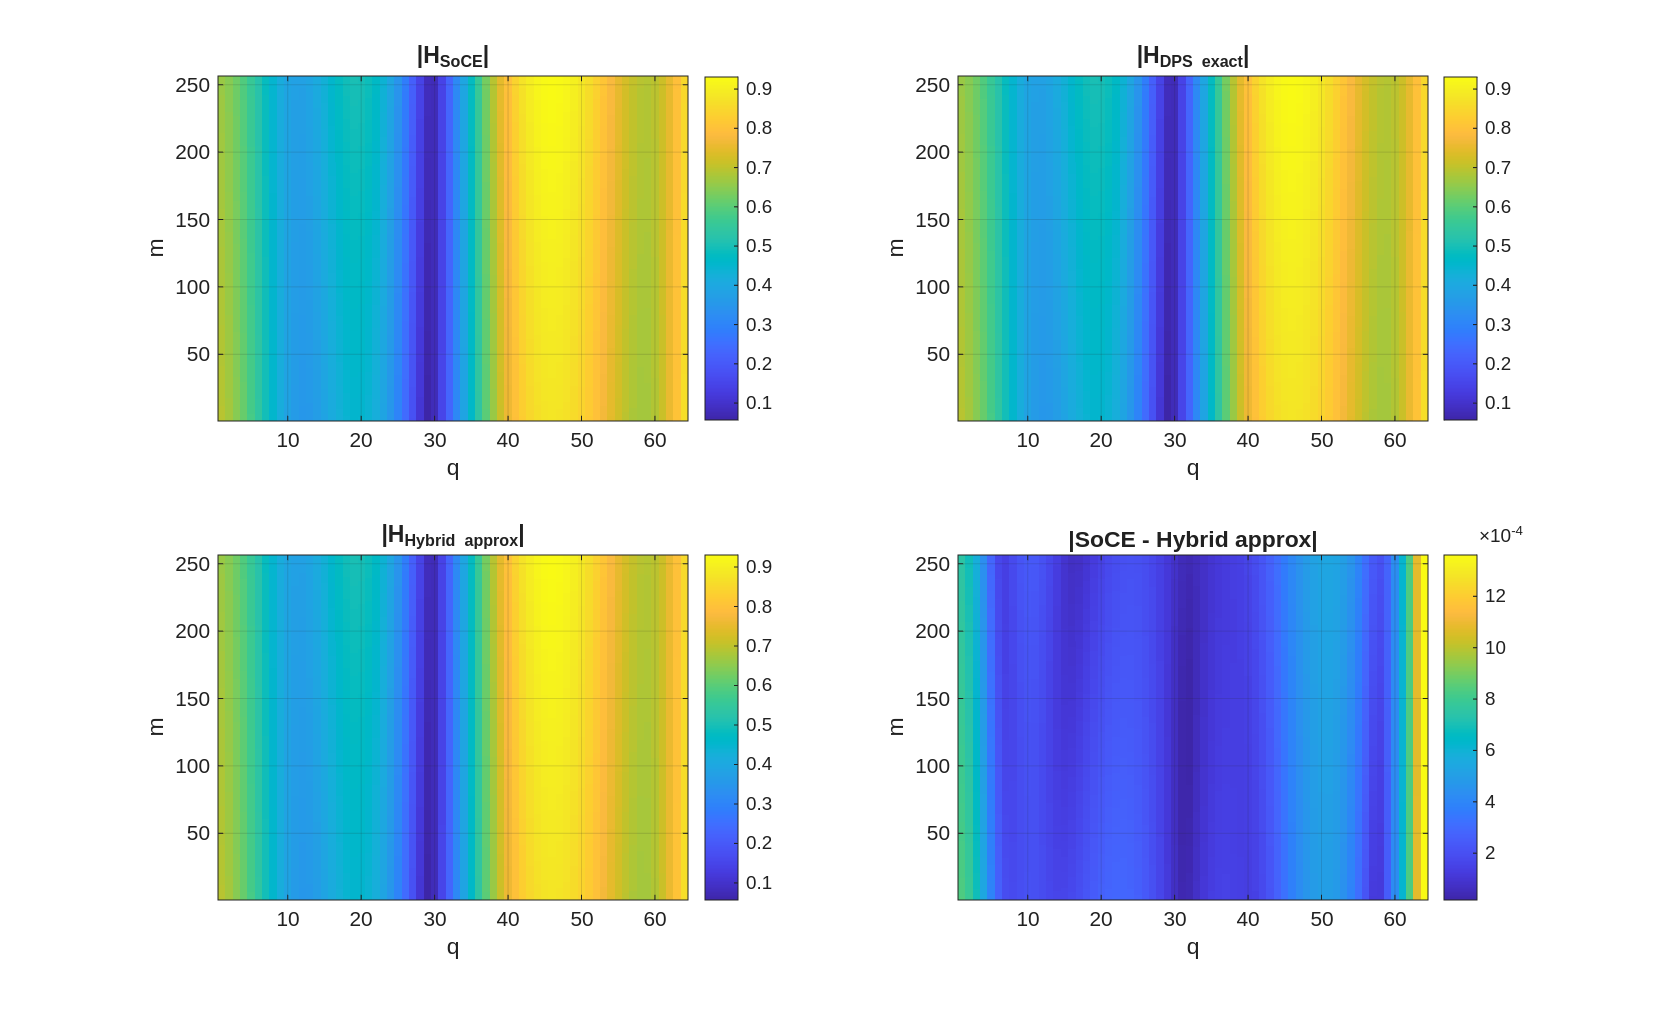
\includegraphics[width=0.9\textwidth]{results/figures/mimo_dps_kaltenberger_approx_tx1_rx1.png}
    \caption{So sánh đáp ứng kênh giữa SoCE, DPS chính xác và phương pháp hybrid cho cặp anten phát--thu thứ nhất}
    \label{fig:mimo_dps_kaltenberger_approx_tx1_rx1}
\end{figure}

Hình~\ref{fig:mimo_dps_kaltenberger_approx_tx1_rx1} cho thấy đáp ứng tái tạo bằng DPS chính xác có dạng biên độ gần với SoCE tham chiếu. Phương pháp hybrid cũng giữ được các vùng biên độ lớn, nhỏ và xu hướng biến thiên theo tần số. Trong cấu hình này, tích \(M\nu_{\mathrm{D,max}}\) nhỏ nên pha Doppler chỉ thay đổi ít trên một khối; vì vậy, biên độ quan sát được biến thiên yếu theo chỉ số thời gian \(m\). Ô sai số tuyệt đối ở góc dưới bên phải giúp xác định vị trí sai khác, nhưng hình ảnh của một cặp anten chưa đủ để đánh giá toàn bộ tensor kênh. Vì vậy, phần tiếp theo sử dụng MSE, NMSE và sai số cực đại được tính trên tất cả mẫu thời gian, tần số và cặp anten.

\subsection{Kết quả sai số và thời gian chạy}
\label{subsec:ch4_error_runtime}

Ba chỉ tiêu sai số cung cấp ba cách nhìn bổ sung. MSE là trung bình bình phương độ lớn sai số trên toàn bộ tensor; sai số tuyệt đối lớn nhất cho biết trường hợp lệch nhiều nhất tại một phần tử; còn NMSE chuẩn hóa MSE theo công suất trung bình của kênh tham chiếu. Nhờ phép chuẩn hóa, NMSE là đại lượng không có đơn vị và thuận tiện để so sánh giữa các nhánh. Với kênh tham chiếu \(H_{\mathrm{SoCE}}\) và kênh tái tạo \(\hat{H}\), NMSE được xác định bởi:
\begin{equation}
\mathrm{NMSE}
=
\frac{\mathbb{E}\{|H_{\mathrm{SoCE}}-\hat{H}|^2\}}
{\mathbb{E}\{|H_{\mathrm{SoCE}}|^2\}}.
\label{eq:ch4_nmse_definition}
\end{equation}
Trong \eqref{eq:ch4_nmse_definition}, ký hiệu \(\mathbb{E}\{\cdot\}\) là phép lấy trung bình trên toàn bộ phần tử của khối kênh mô phỏng, không phải trung bình của nhiều lần sinh kênh độc lập. Giá trị NMSE càng gần không thì kênh tái tạo càng gần SoCE theo nghĩa năng lượng sai số.

Hình~\ref{fig:mimo_dps_kaltenberger_approx_nmse_bar} biểu diễn NMSE của ba nhánh DPS theo thang logarit. Trên thang này, mỗi khoảng cách một bậc tương ứng với hệ số mười; do đó, biểu đồ cho phép quan sát rõ các giá trị sai số chênh nhau nhiều bậc độ lớn.

\begin{figure}[H]
    \centering
    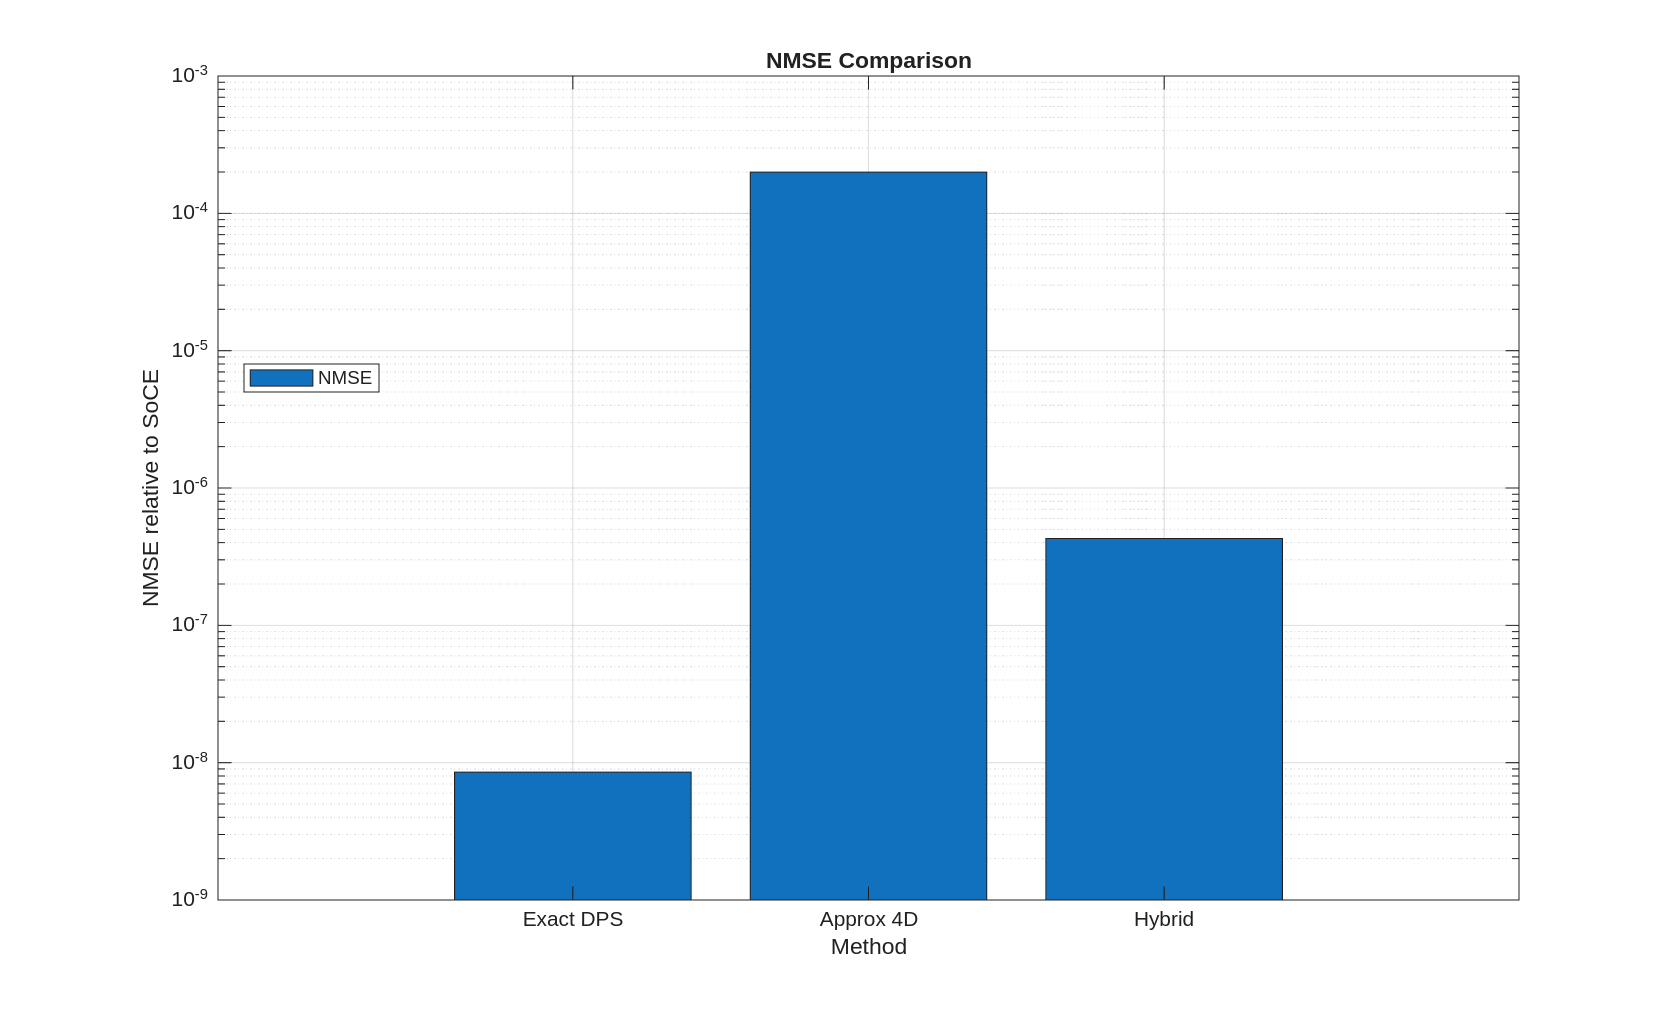
\includegraphics[width=0.9\textwidth]{results/figures/mimo_dps_kaltenberger_approx_nmse_bar.png}
    \caption{So sánh NMSE của các nhánh DPS so với kênh SoCE tham chiếu}
    \label{fig:mimo_dps_kaltenberger_approx_nmse_bar}
\end{figure}

Từ Hình~\ref{fig:mimo_dps_kaltenberger_approx_nmse_bar}, nhánh DPS chính xác có NMSE nhỏ nhất, ở mức \(8{,}53\times10^{-9}\). Nhánh DPS xấp xỉ 4D có NMSE lớn nhất, \(1{,}99\times10^{-4}\). Phương pháp hybrid đạt \(4{,}29\times10^{-7}\), nằm giữa hai nhánh trên nhưng thấp hơn xấp xỉ 4D hơn hai bậc độ lớn. Thứ tự này cho thấy việc tránh xấp xỉ DPS ở hai chiều anten giúp giảm sai số trong cấu hình hiện tại; nguyên nhân của từng nhánh được phân tích riêng ở Mục~\ref{subsec:ch4_branch_discussion}.

Bảng~\ref{tab:ch4_metrics} bổ sung các giá trị MSE, sai số cực đại và hai thành phần thời gian. Cột \(t_{\alpha}\) là thời gian tạo tensor hệ số; cột \(t_{\mathrm{rec}}\) là thời gian tái tạo kênh từ tensor đó. Tổng hai cột là thời gian xử lý của một nhánh DPS sau khi các cơ sở cần thiết đã được tạo.

\begin{table}[H]
    \centering
    \scriptsize
    \setlength{\tabcolsep}{3pt}
    \caption{Sai số và thời gian chạy của các nhánh mô phỏng}
    \label{tab:ch4_metrics}
    \begin{tabularx}{\textwidth}{>{\raggedright\arraybackslash}X c c c c c}
        \toprule
        Nhánh mô phỏng & MSE & NMSE & Max \(|e|\) & \(t_{\alpha}\) (s) & \(t_{\mathrm{rec}}\) (s) \\
        \midrule
        DPS chính xác
        & \(3{,}43\times10^{-9}\)
        & \(8{,}53\times10^{-9}\)
        & \(2{,}01\times10^{-4}\)
        & \(9{,}14\times10^{-3}\)
        & \(8{,}18\times10^{-3}\) \\
        DPS xấp xỉ 4D
        & \(8{,}03\times10^{-5}\)
        & \(1{,}99\times10^{-4}\)
        & \(2{,}23\times10^{-2}\)
        & \(1{,}50\times10^{-2}\)
        & \(6{,}94\times10^{-3}\) \\
        Phương pháp hybrid
        & \(1{,}72\times10^{-7}\)
        & \(4{,}29\times10^{-7}\)
        & \(1{,}67\times10^{-3}\)
        & \(5{,}88\times10^{-3}\)
        & \(1{,}18\times10^{-3}\) \\
        \bottomrule
    \end{tabularx}
\end{table}

Các giá trị trong Bảng~\ref{tab:ch4_metrics} cho thấy MSE, NMSE và sai số tuyệt đối lớn nhất đều xếp ba nhánh theo cùng một thứ tự. Điều này giúp tránh kết luận dựa riêng vào một chỉ tiêu. Về thời gian, nhánh DPS xấp xỉ 4D tốn nhiều thời gian tạo hệ số nhất vì phải xấp xỉ trên cả bốn chiều. Phương pháp hybrid có thời gian tái tạo thấp nhất vì chỉ thực hiện phép tái tạo DPS theo thời gian và tần số; hai chiều anten đã được giữ trực tiếp trong tensor hệ số.

Hình~\ref{fig:mimo_dps_kaltenberger_approx_runtime_bar} so sánh thời gian chạy của SoCE và ba nhánh DPS trong cùng lần mô phỏng. Đối với mỗi nhánh DPS, tổng thời gian gồm thời gian tạo hệ số và thời gian tái tạo trong Bảng~\ref{tab:ch4_metrics}. Thời gian tạo các cơ sở DPS và cơ sở độ phân giải cao được thực hiện trước các lệnh đo thời gian nên chưa được tính trong biểu đồ.

\begin{figure}[H]
    \centering
    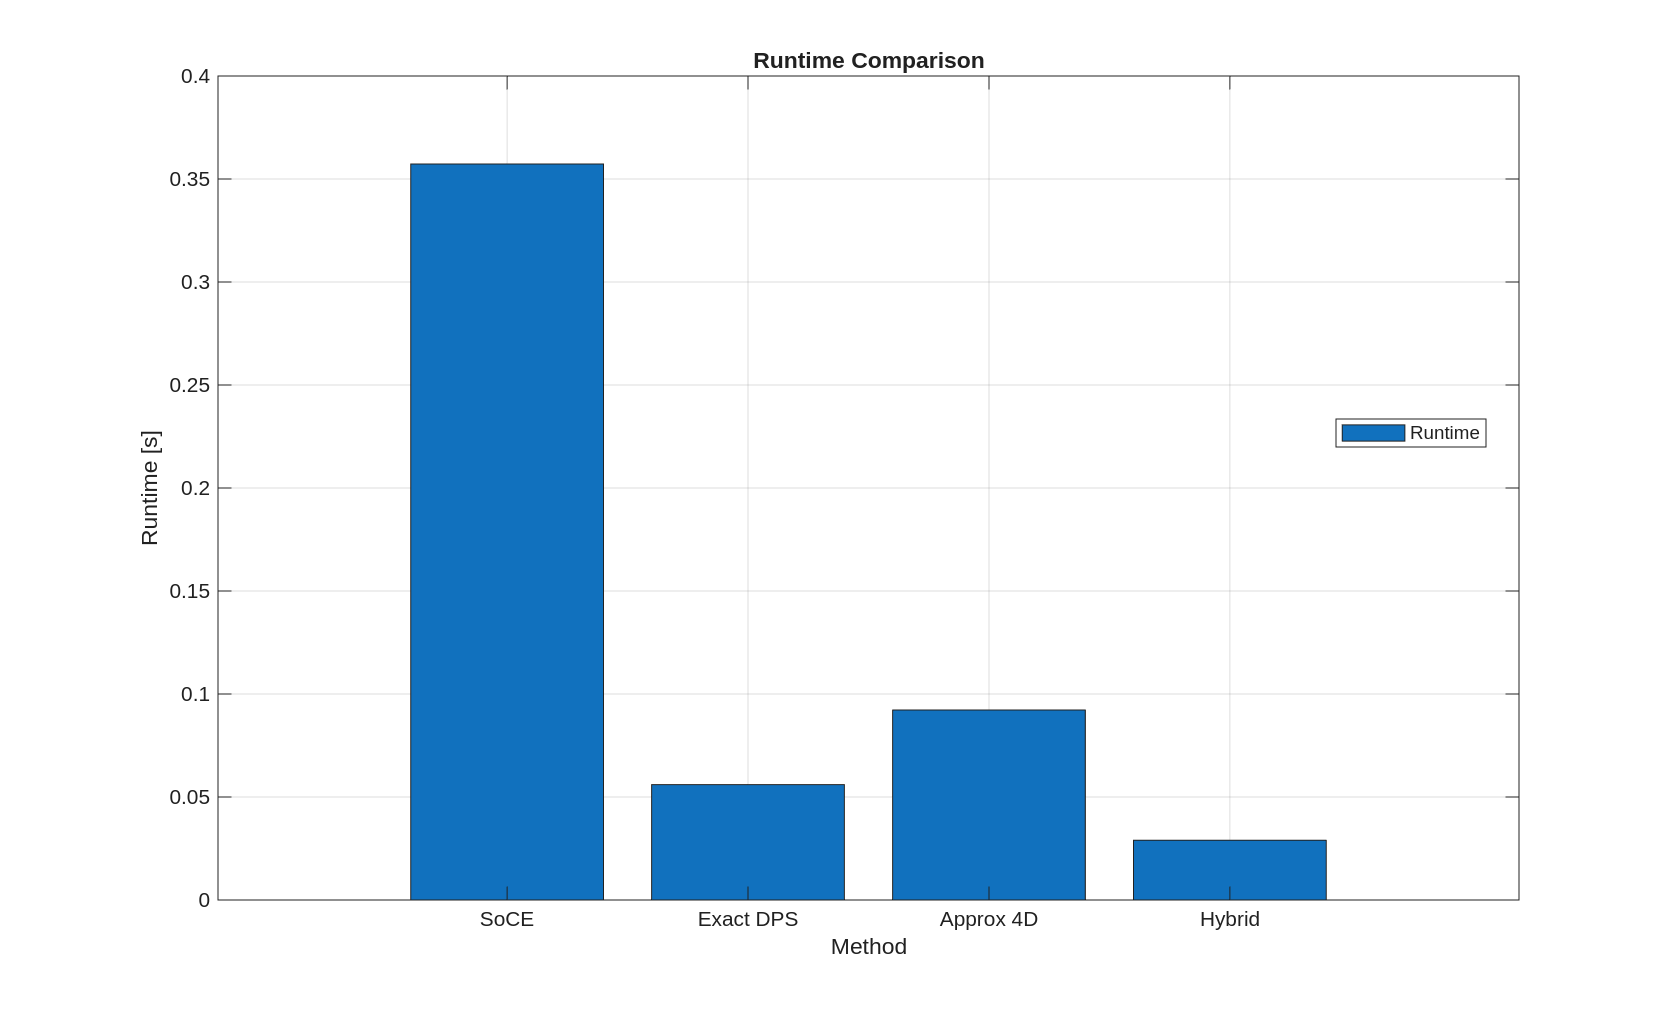
\includegraphics[width=0.9\textwidth]{results/figures/mimo_dps_kaltenberger_approx_runtime_bar.png}
    \caption{So sánh thời gian chạy của SoCE và các nhánh DPS trong cấu hình mô phỏng hiện tại}
    \label{fig:mimo_dps_kaltenberger_approx_runtime_bar}
\end{figure}

Từ Hình~\ref{fig:mimo_dps_kaltenberger_approx_runtime_bar}, thời gian tính SoCE tham chiếu trong lần chạy này là \(0{,}058161\,\mathrm{s}\). Tổng thời gian tạo hệ số và tái tạo của DPS chính xác là khoảng \(0{,}017324\,\mathrm{s}\), của DPS xấp xỉ 4D là khoảng \(0{,}021947\,\mathrm{s}\), và của phương pháp hybrid là khoảng \(0{,}007063\,\mathrm{s}\). Trong phạm vi phép đo này, cả ba tổng thời gian đều nhỏ hơn thời gian SoCE và hybrid có tổng thời gian thấp nhất. Tuy nhiên, kết quả chưa bao gồm chi phí tạo cơ sở DPS, đồng thời còn phụ thuộc vào máy tính, phiên bản MATLAB, cách véc-tơ hóa và cấp phát bộ nhớ. Vì vậy, các số đo chỉ dùng để so sánh các nhánh trong cùng điều kiện chạy, không phải bảo đảm về tốc độ cho mọi cấu hình.

\subsection{Thảo luận từng nhánh mô phỏng}
\label{subsec:ch4_branch_discussion}

Nhánh DPS chính xác trả lời câu hỏi liệu không gian con đã chọn có đủ để chứa phần lớn năng lượng kênh hay không. NMSE \(8{,}53\times10^{-9}\) cho thấy, với \(D_t=6\), \(D_f=9\), \(D_{\mathrm{Tx}}=4\) và \(D_{\mathrm{Rx}}=4\), sai số cắt không gian con ở mức thấp trong cấu hình hiện tại. Kết quả này không có nghĩa DPS tái tạo chính xác tuyệt đối, mà cho thấy phép chiếu chính xác lên số véc-tơ đang giữ gần với SoCE.

Nhánh DPS xấp xỉ 4D trả lời câu hỏi điều gì xảy ra khi không tính các tích vô hướng chính xác. NMSE \(1{,}99\times10^{-4}\) lớn hơn đáng kể so với DPS chính xác vì hệ số được ước lượng từ hàm sóng DPS trên lưới độ phân giải cao. Khi phép xấp xỉ được áp dụng cho cả bốn chiều, sai số hệ số của từng chiều cùng tham gia vào tích tensor. Vì vậy, nhánh này chủ yếu đóng vai trò chẩn đoán ảnh hưởng của công thức xấp xỉ hệ số, chưa phải lựa chọn phù hợp nhất trong cấu hình đang xét.

Phương pháp hybrid trả lời câu hỏi liệu chỉ xấp xỉ hai chiều có kích thước lớn hơn có tạo được cân bằng tốt hơn hay không. Nhánh này đạt NMSE \(4{,}29\times10^{-7}\) so với SoCE và \(4{,}20\times10^{-7}\) so với DPS chính xác. DPS xấp xỉ chỉ được dùng cho thời gian và tần số, còn phần không gian anten được tính trực tiếp bằng hàm mũ. Với \(N_{\mathrm{Tx}}=N_{\mathrm{Rx}}=4\), cách xử lý này tránh sai số xấp xỉ ở hai chiều anten mà vẫn giữ thời gian tái tạo thấp trong phép đo hiện tại. Do đó, hybrid tạo được sự cân bằng phù hợp hơn giữa sai số và thời gian quan sát được trong cấu hình này.

\subsection{Ảnh hưởng của số thành phần đa đường}
\label{subsec:ch4_p_sweep}

Để khảo sát khả năng mở rộng theo số MPC, thí nghiệm quét sử dụng sáu giá trị \(P\in\{10,20,40,80,160,320\}\), trong khi giữ cố định \(M=256\), \(Q=64\), \(N_{\mathrm{Tx}}=N_{\mathrm{Rx}}=4\), \(D_t=6\), \(D_f=9\), \(D_{\mathrm{Tx}}=D_{\mathrm{Rx}}=4\), \(r_t=2\) và \(r_f=512\). Tại mỗi giá trị \(P\), NMSE được đánh giá trên 20 seed. Trong từng seed, các cấu hình dùng chung một tập MPC lồng nhau nhưng trọng số được chuẩn hóa lại theo \(P\) để giữ công suất kỳ vọng xấp xỉ không đổi. Thời gian chạy được đo riêng trên dữ liệu cố định sau bước khởi động, lặp 10 lần và lấy trung vị; thời gian tạo cơ sở DPS không nằm trong phép đo. Thí nghiệm tập trung vào DPS chính xác và phương pháp hybrid vì hai nhánh này lần lượt thể hiện sai số cắt không gian con và phương án xấp xỉ phù hợp hơn cho cấu hình MIMO đang xét.

Hình~\ref{fig:mimo_dps_kaltenberger_p_sweep_nmse} biểu diễn trung vị NMSE và khoảng tứ phân vị từ 20 hiện thực kênh tại mỗi số MPC. Trong toàn bộ dải khảo sát, trung vị NMSE của DPS chính xác nằm trong khoảng từ \(2{,}98\times10^{-9}\) đến \(5{,}90\times10^{-9}\), còn phương pháp hybrid nằm trong khoảng từ \(1{,}67\times10^{-7}\) đến \(2{,}29\times10^{-7}\). Như vậy, thứ tự sai số giữa hai nhánh được duy trì tại cả sáu điểm và trên các khoảng tứ phân vị quan sát được: DPS chính xác có NMSE thấp hơn hybrid trong thí nghiệm này.

\begin{figure}[H]
    \centering
    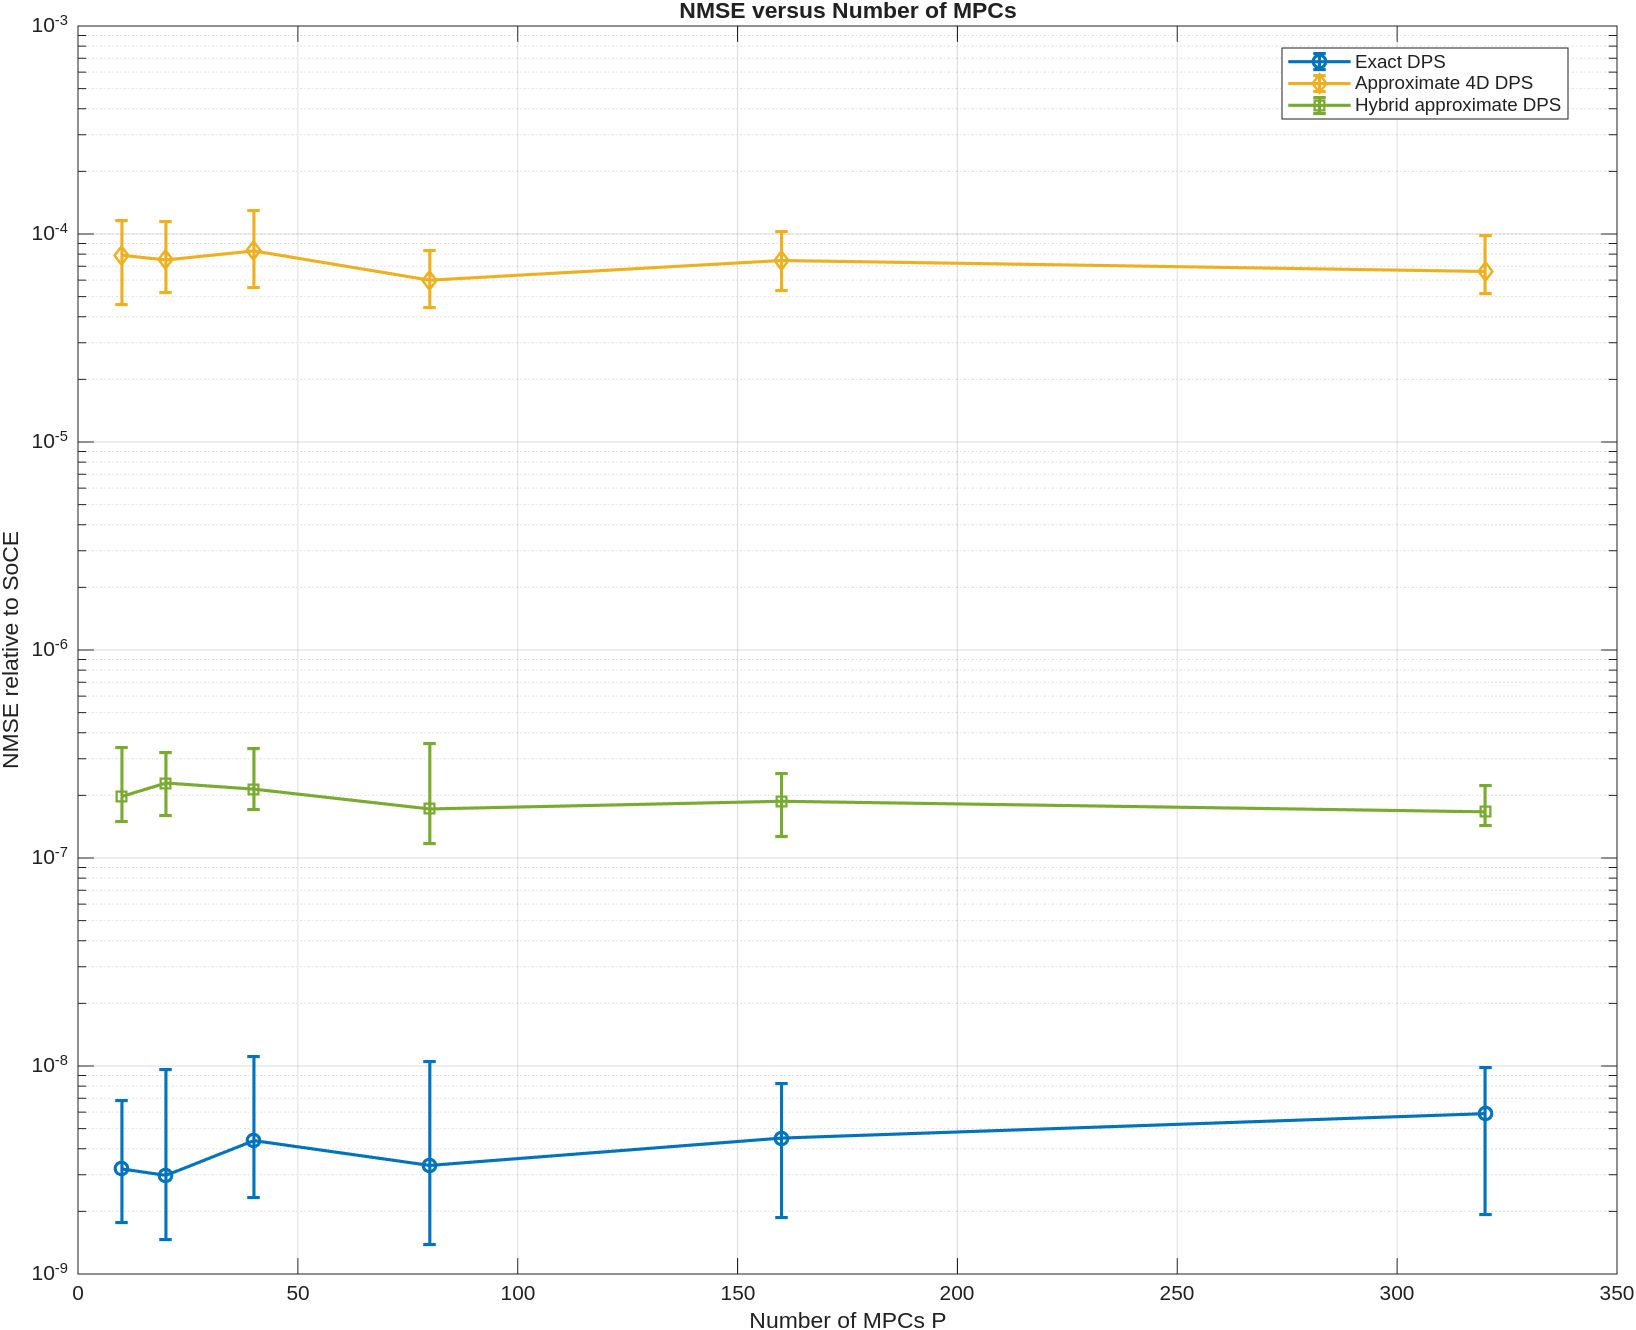
\includegraphics[width=0.9\textwidth]{results/figures/mimo_dps_kaltenberger_p_sweep_nmse.png}
    \caption{NMSE của DPS chính xác và phương pháp hybrid khi thay đổi số MPC}
    \label{fig:mimo_dps_kaltenberger_p_sweep_nmse}
\end{figure}

Các trung vị NMSE không biến thiên đơn điệu theo \(P\), đồng thời các khoảng tứ phân vị của cùng một nhánh chồng lấn đáng kể giữa các giá trị \(P\). Vì NMSE được chuẩn hóa theo công suất của từng kênh tham chiếu và còn phụ thuộc vào vị trí, pha, trọng số MPC, kết quả hiện tại không cho thấy sai số tăng có hệ thống khi số MPC tăng. Kết luận phù hợp trong phạm vi sweep này là số MPC ảnh hưởng ít đến mức NMSE điển hình khi miền giới hạn băng, số chiều DPS và hệ số phân giải được giữ cố định.

Hình~\ref{fig:mimo_dps_kaltenberger_p_sweep_runtime} cho thấy thời gian SoCE tăng rõ khi số MPC lớn. Từ \(P=40\) đến \(P=320\), trung vị thời gian SoCE tăng từ \(0{,}030090\,\mathrm{s}\) lên \(0{,}253762\,\mathrm{s}\). Tại \(P=320\), trung vị tổng thời gian tạo hệ số và tái tạo là \(0{,}015057\,\mathrm{s}\) đối với DPS chính xác và \(0{,}014187\,\mathrm{s}\) đối với hybrid, đều thấp hơn thời gian SoCE trong cùng phép đo. Kết quả này phù hợp với phân tích độ phức tạp: SoCE phải cộng đóng góp của từng MPC trên toàn bộ khối mẫu, trong khi phần tái tạo DPS phụ thuộc chủ yếu vào kích thước cơ sở đã chọn.

\begin{figure}[H]
    \centering
    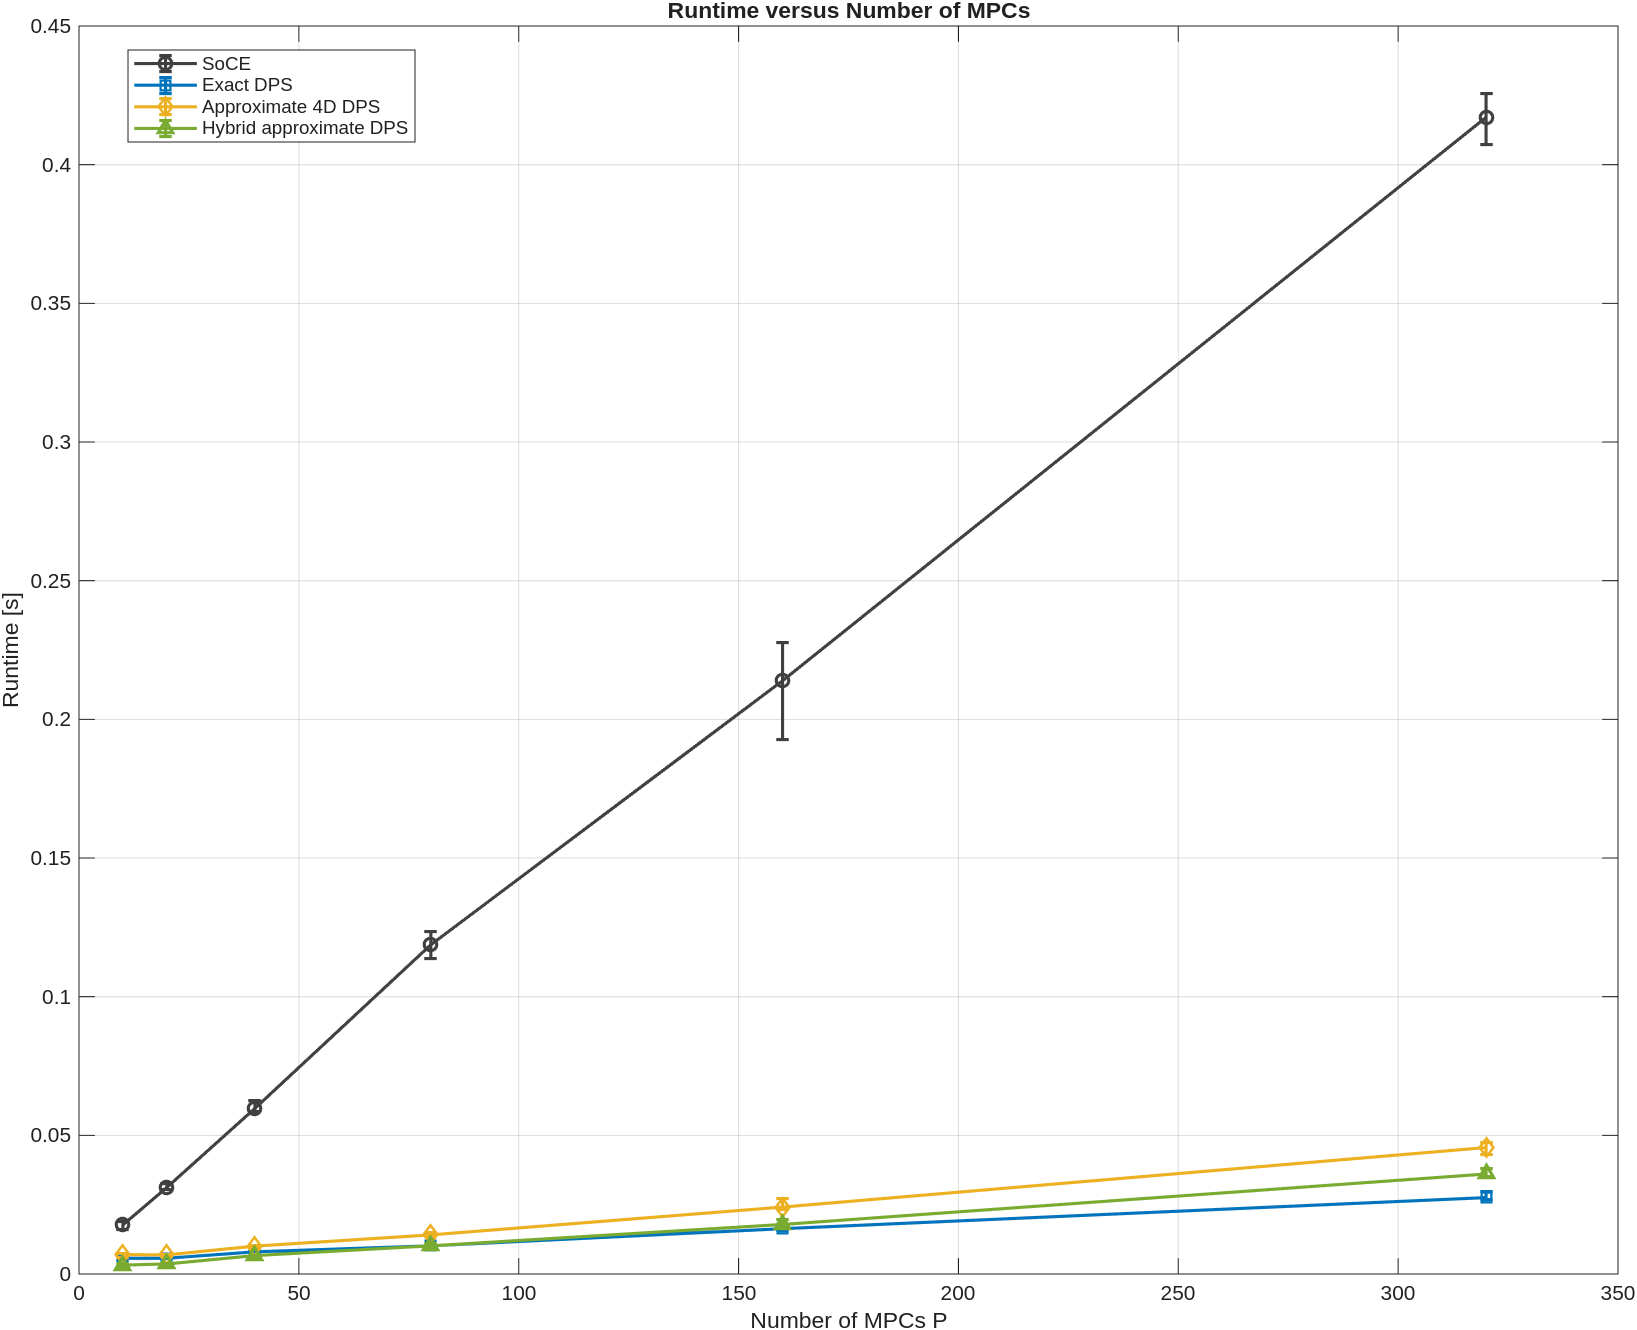
\includegraphics[width=0.9\textwidth]{results/figures/mimo_dps_kaltenberger_p_sweep_runtime.png}
    \caption{Thời gian chạy của SoCE, DPS chính xác và phương pháp hybrid khi thay đổi số MPC}
    \label{fig:mimo_dps_kaltenberger_p_sweep_runtime}
\end{figure}

Các thanh sai số trên Hình~\ref{fig:mimo_dps_kaltenberger_p_sweep_runtime} biểu diễn khoảng tứ phân vị của 10 lần đo. Sau khi có bước khởi động và đo lặp, điểm \(P=10\) không còn biểu hiện thời gian cao bất thường so với các điểm kế tiếp. Tuy nhiên, các số đo vẫn phụ thuộc vào máy tính, phiên bản MATLAB, trạng thái hệ thống và cách triển khai; vì vậy chúng chỉ được dùng để đánh giá xu hướng và so sánh các nhánh trong cùng môi trường thực thi.

\subsection{Benchmark bốn phương pháp và điểm hòa vốn}
\label{subsec:ch4_four_method_benchmark}

Để phân biệt lợi ích do lựa chọn cơ sở với lợi ích do tối ưu cách tạo pha, một benchmark riêng được thực hiện cho bốn phương pháp: SoCE trực tiếp, SoCE đệ quy, CE-BEM và DPS chính xác. Các phương pháp dùng chung khối kênh kích thước \(256\times64\times4\times4\), cùng các tập MPC và cùng số chiều \((6,9,4,4)\) cho hai mô hình khai triển cơ sở. CE-BEM sử dụng các hàm mũ có tần số phân bố đều trong từng miền giới hạn băng và hệ số bình phương tối thiểu; DPS dùng phép chiếu chính xác. Cách thiết lập này giúp so sánh hai cơ sở mà không trộn thêm sai số của công thức hệ số DPS xấp xỉ.

NMSE được tổng hợp trên 20 hiện thực kênh tại mỗi giá trị \(P\), còn thời gian được đo 10 lần trên dữ liệu cố định sau bước khởi động và lấy trung vị. Thời gian xử lý mỗi khối bao gồm bước tạo hệ số và tái tạo, nhưng không gồm bước tạo cơ sở dùng lại. Hình~\ref{fig:ch4_four_method_runtime} cho thấy chi phí của hai nhánh SoCE tăng rõ theo số MPC, trong khi thời gian của CE-BEM và DPS tăng chậm hơn trong dải khảo sát.

\begin{figure}[H]
    \centering
    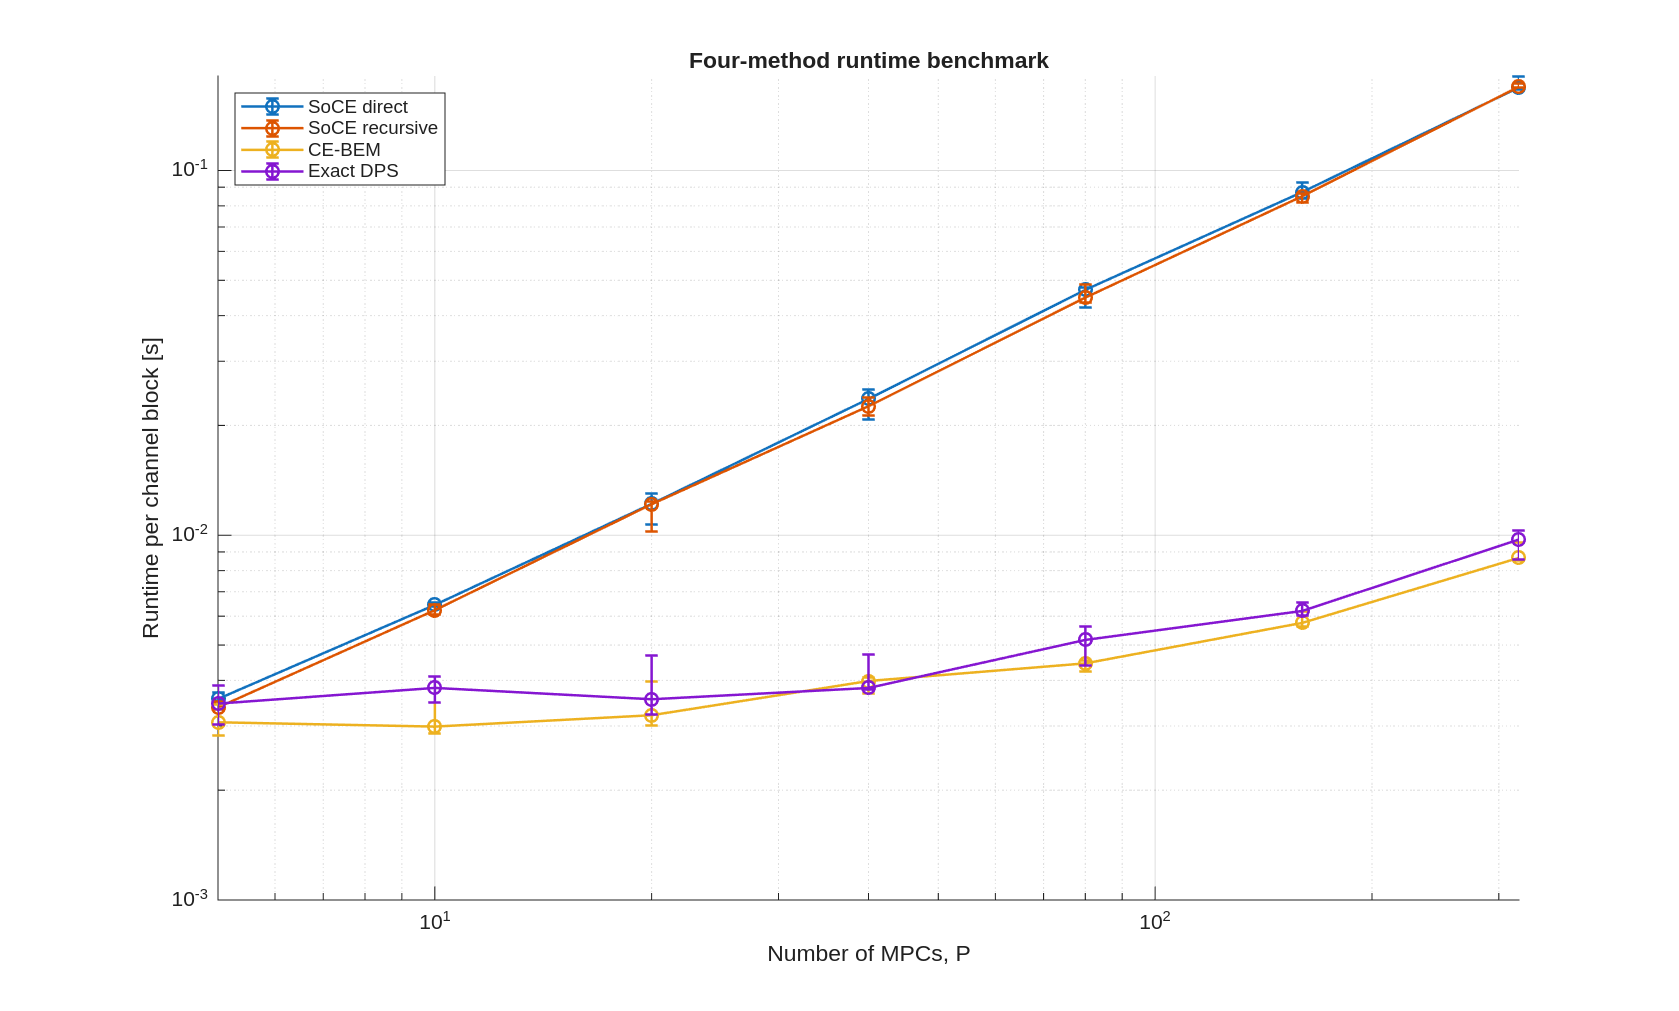
\includegraphics[width=0.9\textwidth]{results/figures/mimo_four_method_benchmark_runtime.png}
    \caption{Thời gian xử lý mỗi khối của bốn phương pháp khi thay đổi số MPC}
    \label{fig:ch4_four_method_runtime}
\end{figure}

Tại \(P=80\), Bảng~\ref{tab:ch4_four_method_p80} cho thấy SoCE đệ quy có thời gian gần SoCE trực tiếp và các khoảng tứ phân vị còn chồng lấn. Do đó, phép cập nhật pha đệ quy không tạo ra lợi thế thời gian rõ ràng trong cách cài đặt MATLAB hiện tại, dù NMSE của nó chỉ ở mức sai số làm tròn. CE-BEM và DPS chính xác lần lượt đạt hệ số tăng tốc khoảng \(10{,}57\) và \(9{,}12\) so với SoCE trực tiếp. DPS có NMSE trung vị thấp hơn CE-BEM gần một bậc độ lớn, lần lượt là \(3{,}33\times10^{-9}\) và \(2{,}96\times10^{-8}\). Kết quả không khẳng định CE-BEM luôn nhanh hơn DPS, vì thời gian còn phụ thuộc cách chọn cơ sở, phép nhân ma trận và khả năng khai thác FFT.

\begin{table}[H]
    \centering
    \small
    \caption{Benchmark bốn phương pháp tại \(P=80\)}
    \label{tab:ch4_four_method_p80}
    \begin{tabular}{lccc}
        \toprule
        Phương pháp & Thời gian trung vị (s) & NMSE trung vị & Tăng tốc ($\times$) \\
        \midrule
        SoCE trực tiếp & \(4{,}708\times10^{-2}\) & \(0\) & \(1{,}00\) \\
        SoCE đệ quy & \(4{,}482\times10^{-2}\) & \(3{,}05\times10^{-29}\) & \(1{,}05\) \\
        CE-BEM & \(4{,}454\times10^{-3}\) & \(2{,}96\times10^{-8}\) & \(10{,}57\) \\
        DPS chính xác & \(5{,}164\times10^{-3}\) & \(3{,}33\times10^{-9}\) & \(9{,}12\) \\
        \bottomrule
    \end{tabular}
\end{table}

Hình~\ref{fig:ch4_four_method_nmse} xác nhận thứ tự sai số của hai mô hình khai triển cơ sở được duy trì trên dải \(P=5\)--\(320\). NMSE không tăng đơn điệu theo \(P\), phù hợp với việc sai số chủ yếu do mức độ phù hợp của không gian con với vị trí tần số MPC, thay vì chỉ do số lượng MPC.

\begin{figure}[H]
    \centering
    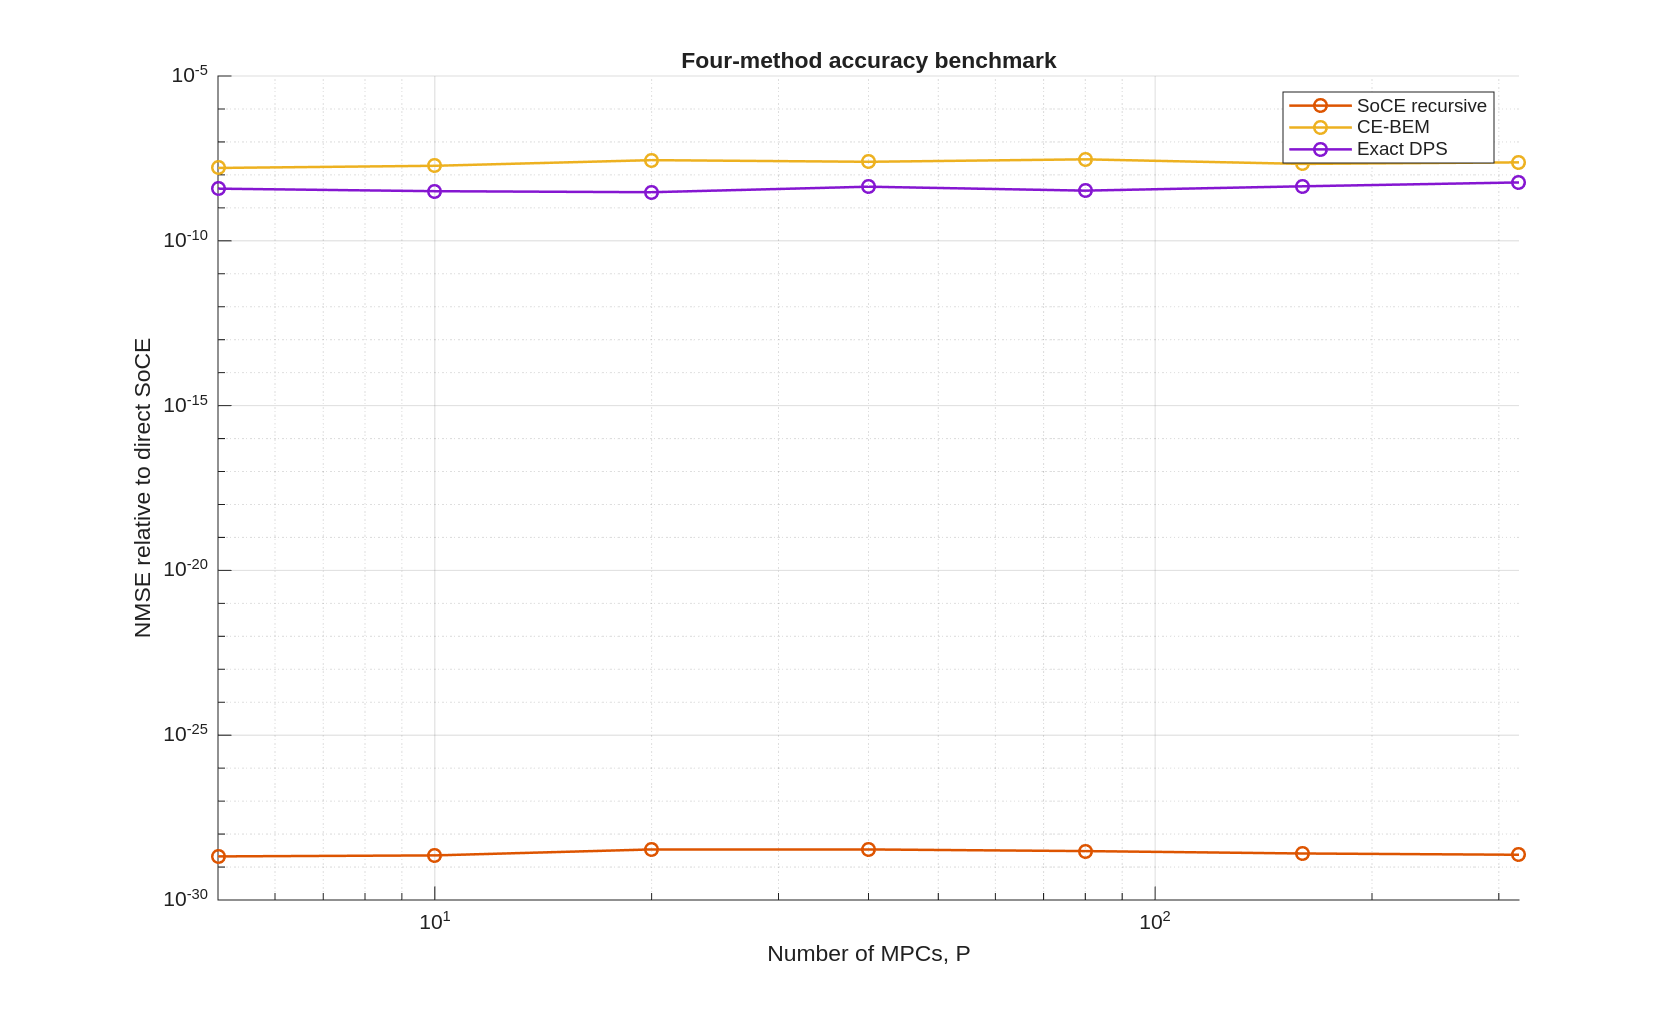
\includegraphics[width=0.9\textwidth]{results/figures/mimo_four_method_benchmark_nmse.png}
    \caption{NMSE của SoCE đệ quy, CE-BEM và DPS chính xác so với SoCE trực tiếp}
    \label{fig:ch4_four_method_nmse}
\end{figure}

Điểm hòa vốn thứ nhất được xác định theo số MPC: đó là giá trị mà thời gian xử lý mỗi khối của phương pháp đang xét chuyển từ lớn hơn sang nhỏ hơn SoCE trực tiếp và duy trì nhỏ hơn tại các điểm khảo sát tiếp theo. Trong lần đo hiện tại, CE-BEM và DPS chính xác đã nhanh hơn SoCE trực tiếp tại điểm nhỏ nhất \(P=5\) và duy trì thứ tự này đến \(P=320\). Vì sweep không chứa giá trị nhỏ hơn 5, kết quả chỉ xác định được điểm hòa vốn thực nghiệm thỏa \(P_{\mathrm{BE}}\le5\), chưa định vị chính xác giao điểm. Đối với SoCE đệ quy, chênh lệch nhỏ và khoảng tứ phân vị chồng lấn nên chưa đủ cơ sở xác lập một điểm hòa vốn ổn định.

Điểm hòa vốn thứ hai xét chi phí tiền xử lý. Thời gian tạo cơ sở đo được là \(0{,}0139\,\mathrm{s}\) cho CE-BEM và \(0{,}2264\,\mathrm{s}\) cho DPS. Tại \(P=80\), lấy chi phí tiền xử lý chia cho phần thời gian tiết kiệm trên mỗi khối cho thấy CE-BEM hòa vốn từ khối đầu tiên, còn DPS cần khoảng 6 khối. Sau ngưỡng này, cơ sở được tái sử dụng và lợi ích thời gian tích lũy theo số khối xử lý. Phân tích này giả thiết miền giới hạn băng và kích thước khối không đổi giữa các khối; nếu các tham số đó thay đổi, cơ sở phải được tạo lại và điểm hòa vốn cũng thay đổi.

Có thể biểu diễn lập luận trên dưới dạng tổng thời gian cho \(L\) khối kênh. Gọi \(T_{\mathrm{setup},a}\) là thời gian tiền xử lý và \(T_{\mathrm{block},a}\) là thời gian xử lý một khối của phương pháp \(a\). Khi cơ sở được tái sử dụng, tổng thời gian là:
\begin{equation}
T_a(L)
=T_{\mathrm{setup},a}+L T_{\mathrm{block},a}.
\label{eq:ch4_amortized_runtime}
\end{equation}
Với SoCE trực tiếp, có thể xem \(T_{\mathrm{setup,SoCE}}=0\). Nếu \(T_{\mathrm{block},a}<T_{\mathrm{block,SoCE}}\), số khối nguyên nhỏ nhất để phương pháp \(a\) không còn chậm hơn SoCE được xác định bởi:
\begin{equation}
L_{\mathrm{BE},a}
=\left\lceil
\frac{T_{\mathrm{setup},a}}
{T_{\mathrm{block,SoCE}}-T_{\mathrm{block},a}}
\right\rceil.
\label{eq:ch4_break_even_blocks}
\end{equation}
Phương trình \eqref{eq:ch4_break_even_blocks} cũng cho thấy hai trường hợp không có điểm hòa vốn hữu hạn: thời gian mỗi khối của phương pháp mới bằng hoặc lớn hơn SoCE, hoặc cơ sở phải tạo lại cho từng khối nên không thể phân bổ chi phí tiền xử lý. Do đó, điểm hòa vốn không chỉ phụ thuộc tốc độ tái tạo mà còn phụ thuộc cách hệ thống tổ chức các khối kênh và mức độ ổn định của miền giới hạn băng.

\subsection{Ý nghĩa của kết quả đối với lựa chọn phương pháp}
\label{subsec:ch4_method_selection_implications}

Các kết quả cho thấy không có một nhánh duy nhất tối ưu đồng thời cho mọi mục tiêu. Nếu ưu tiên kiểm tra độ chính xác của không gian con và chấp nhận chi phí chiếu, DPS chính xác là đối chứng phù hợp vì nó tách sai số cắt khỏi sai số xấp xỉ hệ số. Nếu ưu tiên thời gian xử lý trên cấu hình anten nhỏ đang xét, phương pháp hybrid có lợi thế thực dụng: hai chiều lớn hơn được nén bằng DPS, trong khi hai chiều không gian được giữ trực tiếp để tránh xấp xỉ không cần thiết. DPS xấp xỉ 4D vẫn hữu ích như một nhánh chẩn đoán, bởi nó cho thấy hệ quả của việc áp dụng cùng một cơ chế xấp xỉ lên tất cả các chiều mà không xét kích thước và băng thông riêng của từng chiều.

Benchmark với CE-BEM bổ sung một góc nhìn khác. Việc CE-BEM đạt thời gian thấp trong phép đo hiện tại cho thấy phần lợi ích không chỉ đến từ riêng cơ sở DPS, mà còn đến từ việc chuyển kênh sang một không gian hệ số có kích thước nhỏ. Tuy nhiên, với cùng số chiều, DPS đạt NMSE thấp hơn trong dải khảo sát. Kết quả này phù hợp với vai trò khác nhau của hai cơ sở: CE-BEM thuận lợi về cấu trúc Fourier và khả năng triển khai nhanh, còn DPS được xây dựng để tập trung năng lượng của tín hiệu giới hạn băng trên khối hữu hạn. Lựa chọn giữa chúng vì vậy cần dựa trên ngân sách sai số, khả năng dùng FFT và tần suất tái sử dụng cơ sở, thay vì chỉ dựa vào một lần đo thời gian.

Đối với một bộ mô phỏng kênh dùng nhiều lần, quy trình lựa chọn có thể bắt đầu từ miền băng và kích thước khối. Nếu tích thời gian--băng thông cho số chiều DPS gần bằng kích thước đầy đủ, SoCE hoặc CE-BEM có thể đơn giản hơn. Nếu số chiều thiết yếu nhỏ và cơ sở được dùng lại qua nhiều khối, DPS có điều kiện thuận lợi để bù chi phí tiền xử lý. Sau đó, số chiều cần được chọn theo ngưỡng sai số, và nhánh hybrid nên được xem xét khi các chiều anten quá ngắn để việc nén tiếp tục mang lại lợi ích đáng kể. Cách lựa chọn theo từng bước này phản ánh đúng bản chất đánh đổi giữa độ chính xác, thời gian và bộ nhớ đã phân tích trong đồ án.

\subsection{Giới hạn của kết quả hiện tại}
\label{subsec:ch4_limitations}

Các kết quả trong chương này vẫn có một số giới hạn. Thứ nhất, dù các sweep đã dùng 20 seed, các kết quả ở cấu hình chính và các nhánh xấp xỉ 4D vẫn dựa trên phạm vi tham số hẹp, chưa đại diện cho mọi phân bố kênh. Thứ hai, số chiều DPS và hệ số phân giải được chọn theo quy tắc hiện tại của chương trình, chưa tối ưu tự động theo một ngưỡng sai số đặt trước. Thứ ba, phép đo thời gian dùng một tập dữ liệu cố định và phụ thuộc vào môi trường thực thi, do đó chỉ nên dùng để so sánh tương đối trong cùng điều kiện đo. Benchmark bốn phương pháp đã báo riêng chi phí tạo cơ sở, nhưng chưa khảo sát trường hợp miền giới hạn băng thay đổi làm cơ sở phải được cập nhật thường xuyên.

Ngoài ra, mô phỏng hiện tại chưa khớp lại đầy đủ một hình hoặc bảng cụ thể trong bài báo Kaltenberger với toàn bộ tham số tương ứng. Vì vậy, các kết luận từ Bảng~\ref{tab:ch4_metrics} nên được diễn đạt trong phạm vi cấu hình hiện tại: DPS chính xác kiểm chứng tốt không gian con, nhánh DPS xấp xỉ 4D cho thấy ảnh hưởng của xấp xỉ hệ số, và phương pháp hybrid là lựa chọn phù hợp hơn để thảo luận cho kênh MIMO băng rộng trong mô phỏng này.

\subsection{Kết luận chương}
\label{subsec:ch4_conclusion}

Chương này đã trình bày kết quả mô phỏng và phân tích sai số, thời gian tính toán của các nhánh biểu diễn kênh. Trong cấu hình hiện tại, DPS chính xác đạt sai số nhỏ so với SoCE, cho thấy cơ sở DPS đã chọn phù hợp để kiểm chứng biểu diễn không gian con. Nhánh DPS xấp xỉ 4D có sai số lớn hơn do áp dụng xấp xỉ hệ số trên cả bốn chiều. Phương pháp hybrid đạt NMSE \(4{,}29\times10^{-7}\) so với SoCE và có thời gian tái tạo nhỏ trong lần chạy hiện tại, do đó là nhánh chính để thảo luận về mô phỏng MIMO băng rộng có độ phức tạp thấp. Benchmark bổ sung cho thấy CE-BEM và DPS chính xác đều giảm thời gian xử lý mỗi khối trong dải \(P\) đã khảo sát, trong khi DPS duy trì NMSE thấp hơn CE-BEM với cùng số chiều cơ sở trong thí nghiệm này. Phân tích điểm hòa vốn đồng thời chỉ ra rằng lợi ích thực tế còn phụ thuộc khả năng tái sử dụng chi phí tiền xử lý. Các kết quả này được tổng hợp cùng những hạn chế và hướng phát triển trong phần kết luận của đồ án.

\cleardoublepage

    \chaptercustom{5}{KẾT LUẬN VÀ HƯỚNG PHÁT TRIỂN}
\setcounter{section}{5}
\label{chap:conclusion_future}

\subsection{Kết luận chung}
\label{subsec:ch5_general_conclusion}

Đồ án đã nghiên cứu bài toán biểu diễn và tính toán kênh MIMO băng rộng biến thiên theo thời gian dựa trên mô hình kênh hình học. Trong mô hình này, đáp ứng kênh được biểu diễn bằng tổng các hàm mũ phức theo các thành phần đa đường. Cách biểu diễn SoCE giữ được ý nghĩa vật lý rõ ràng vì mỗi MPC tương ứng với một đóng góp theo Doppler, trễ truyền, góc phát và góc thu. Tuy nhiên, khi số mẫu thời gian, số mẫu tần số, số anten và số MPC tăng, việc tính trực tiếp SoCE yêu cầu cộng đóng góp của tất cả MPC tại từng điểm mẫu của khối kênh. Đây là nút thắt chính về độ phức tạp đã được đặt ra ở Chương 1 và phân tích chi tiết hơn ở Chương 2.

Lý do sử dụng DPS trong đồ án xuất phát từ cấu trúc giới hạn băng của kênh. Trên một khối mẫu hữu hạn, các chiều Doppler, trễ, AoD và AoA không tạo ra một tín hiệu tùy ý mà bị giới hạn trong các miền tần số chuẩn hóa xác định bởi tham số vật lý của hệ thống. DPS là cơ sở phù hợp cho tín hiệu giới hạn băng trên tập chỉ số hữu hạn, do đó có thể chuyển bài toán từ tính trực tiếp từng MPC tại từng mẫu sang biểu diễn kênh trong một không gian con có số chiều nhỏ hơn. Cách tiếp cận này phù hợp với định hướng của Kaltenberger và cộng sự về mô hình kênh hình học có độ phức tạp thấp \cite{Kaltenberger2007}.

\subsection{Kết quả đạt được}
\label{subsec:ch5_obtained_results}

Về mặt trình bày lý thuyết, đồ án đã làm rõ quan hệ giữa SoCE và DPS. SoCE được dùng như mô hình tham chiếu trực tiếp, còn DPS được xem như biểu diễn không gian con dựa trên tính giới hạn băng của kênh. Đồ án cũng phân biệt rõ ba mức sử dụng DPS: phép chiếu DPS chính xác, hệ số DPS xấp xỉ bằng hàm sóng trong bốn chiều, và phương pháp hybrid dùng DPS xấp xỉ cho hai chiều thời gian--tần số kết hợp với tính trực tiếp phần không gian anten.

Về mặt triển khai MATLAB, đồ án đã xây dựng và sử dụng các nhánh mô phỏng sau:
\begin{itemize}
    \item SoCE tham chiếu, dùng để tạo khối kênh chuẩn trong cùng cấu hình mô phỏng;
    \item DPS chính xác, dùng phép chiếu chính xác lên cơ sở DPS để kiểm chứng sai số cắt không gian con;
    \item DPS xấp xỉ 4D, dùng công thức xấp xỉ hệ số DPS cho cả bốn chiều;
    \item phương pháp hybrid, dùng DPS xấp xỉ cho thời gian và tần số, còn phần không gian anten được tính bằng hàm mũ trực tiếp.
\end{itemize}

Trong cấu hình mô phỏng hiện tại với \(M=256\), \(Q=64\), \(N_{\mathrm{Tx}}=N_{\mathrm{Rx}}=4\), \(P=80\) và \(D_{\mathrm{total}}=864\), nhánh DPS chính xác đạt NMSE \(8{,}53\times10^{-9}\) so với SoCE. Giá trị này cho thấy số chiều DPS đã chọn đủ để biểu diễn khối kênh với sai số cắt không gian con nhỏ trong cấu hình đang xét. Nhánh DPS xấp xỉ 4D đạt NMSE \(1{,}99\times10^{-4}\), phản ánh sai số tăng lên khi xấp xỉ hệ số được áp dụng đồng thời ở cả bốn chiều. Phương pháp hybrid đạt NMSE \(4{,}29\times10^{-7}\) so với SoCE và \(4{,}20\times10^{-7}\) so với DPS chính xác. Kết quả này cho thấy, trong mô phỏng hiện tại, hybrid là nhánh phù hợp hơn để thảo luận cho kênh MIMO băng rộng vì tránh xấp xỉ hệ số ở hai chiều không gian anten trong khi vẫn khai thác được biểu diễn DPS ở hai chiều thời gian--tần số.

Các kết quả thời gian chạy cũng thống nhất với phân tích định tính về độ phức tạp. Trong cùng một lần chạy MATLAB, thời gian tính SoCE tham chiếu là \(0{,}222372\,\mathrm{s}\), trong khi tổng thời gian tạo hệ số và tái tạo của phương pháp hybrid là khoảng \(0{,}025322\,\mathrm{s}\). Các giá trị này chỉ nên được hiểu là số đo tham khảo trong cùng môi trường chạy, nhưng chúng minh họa được xu hướng giảm khối lượng tính toán khi số chiều DPS nhỏ hơn đáng kể số mẫu của toàn khối kênh.

\subsection{Hạn chế của đồ án}
\label{subsec:ch5_limitations}

Các kết quả trong đồ án vẫn còn một số hạn chế. Thứ nhất, mô phỏng hiện tại chưa khớp lại đầy đủ một hình hoặc bảng cụ thể trong bài báo Kaltenberger với toàn bộ tham số tương ứng. Vì vậy, kết quả hiện tại chủ yếu có vai trò kiểm chứng mô hình và so sánh các nhánh triển khai trong cùng một cấu hình, chưa phải là tái tạo hoàn chỉnh kết quả gốc của bài báo.

Thứ hai, cấu hình mô phỏng đang dùng còn nhỏ hơn các cấu hình lớn thường xuất hiện trong phân tích độ phức tạp của hệ thống MIMO băng rộng. Việc dùng \(N_{\mathrm{Tx}}=N_{\mathrm{Rx}}=4\) giúp kiểm soát bộ nhớ và thời gian chạy trong MATLAB, nhưng chưa phản ánh đầy đủ lợi ích hoặc chi phí của DPS khi số anten và kích thước khối kênh tăng mạnh.

Thứ ba, số chiều DPS \(D\) và các hệ số phân giải \(r\) trong script hiện tại được chọn theo quy tắc kinh nghiệm. Đồ án chưa triển khai cơ chế tự động chọn các tham số này theo một ngưỡng sai số hoặc ngưỡng bias \(E_{\max}\). Do đó, quan hệ giữa lựa chọn \(D\), lựa chọn \(r\), sai số NMSE và chi phí tính toán mới được đánh giá ở mức một cấu hình cụ thể.

Thứ tư, thời gian chạy MATLAB chưa đại diện cho một triển khai phần cứng hoặc một thư viện tối ưu hóa chuyên dụng. Kết quả thời gian phụ thuộc vào máy tính, phiên bản MATLAB, cách vector hóa và chi phí cấp phát bộ nhớ. Vì vậy, các số đo này chỉ nên dùng để so sánh tương đối giữa các nhánh trong cùng lần chạy.

\subsection{Hướng phát triển}
\label{subsec:ch5_future_work}

Hướng phát triển trực tiếp đầu tiên là thực hiện quét tham số theo số chiều DPS \(D\) và hệ số phân giải \(r\). Việc này cho phép xây dựng đường cong đánh đổi giữa NMSE, số hệ số cần lưu và thời gian chạy. Khi có kết quả quét tham số, đồ án có thể chuyển từ nhận xét trên một cấu hình riêng lẻ sang phân tích có hệ thống hơn về vùng hoạt động phù hợp của DPS.

Hướng thứ hai là tăng kích thước mô phỏng nếu điều kiện bộ nhớ cho phép. Các cấu hình với nhiều anten hơn, nhiều mẫu tần số hơn hoặc số MPC lớn hơn sẽ làm rõ hơn khác biệt giữa cách tính SoCE trực tiếp và biểu diễn dựa trên DPS. Đây cũng là bước cần thiết để đánh giá tốt hơn phương pháp hybrid trong bối cảnh MIMO băng rộng quy mô lớn.

Hướng thứ ba là tái tạo một hình hoặc bảng độ phức tạp trong bài báo gốc với tham số được khớp đầy đủ. Việc này giúp kiểm chứng trực tiếp hơn giữa mã mô phỏng của đồ án và kết quả trong tài liệu tham khảo. Sau bước này, các nhận xét định lượng về độ phức tạp và sai số có thể được đặt trên cơ sở so sánh chặt chẽ hơn.

Hướng thứ tư là chuẩn hóa mã MATLAB thành các hàm độc lập và có giao diện tham số rõ ràng. Các khối như sinh MPC, tính SoCE, tạo cơ sở DPS, tính hệ số DPS chính xác, tính hệ số xấp xỉ và tái tạo hybrid nên được tách thành các hàm có thể tái sử dụng. Cách tổ chức này giúp mở rộng mô phỏng, giảm rủi ro sai lệch ký hiệu và thuận tiện hơn cho việc kiểm thử.

Cuối cùng, có thể khảo sát thêm các phân bố MPC không đều hoặc các kịch bản kênh gần với tiêu chuẩn thực tế hơn. Trong mô phỏng hiện tại, MPC được sinh đều trong miền giới hạn băng để kiểm tra tính chất của biểu diễn DPS. Các phân bố tập trung theo cụm, phân bố theo góc không đều hoặc mô hình công suất trễ phức tạp hơn sẽ giúp đánh giá tính ổn định của phương pháp trong điều kiện kênh thực tế hơn.

\subsection{Kết luận chương}
\label{subsec:ch5_conclusion}

Chương này đã tổng kết toàn bộ đồ án theo mạch lập luận từ SoCE trực tiếp đến biểu diễn DPS và triển khai MATLAB. Trong phạm vi mô phỏng hiện tại, DPS chính xác kiểm chứng tốt không gian con DPS, DPS xấp xỉ 4D cho thấy ảnh hưởng của xấp xỉ hệ số khi áp dụng ở cả bốn chiều, còn phương pháp hybrid đạt sai số nhỏ so với SoCE và có chi phí tái tạo thấp trong cùng lần chạy. Kết quả này ủng hộ việc dùng DPS như một công cụ giảm độ phức tạp cho mô phỏng kênh MIMO băng rộng, đồng thời cho thấy cần tiếp tục mở rộng mô phỏng và khớp tham số với bài báo gốc để củng cố kết luận định lượng.

\cleardoublepage

    % KẾT THÚC
    \phantomsection\section*{\centering KẾT LUẬN}
\addcontentsline{toc}{section}{\numberline{}KẾT LUẬN}

\phantomsection\subsection*{Kết luận chung}
\addcontentsline{toc}{section}{\numberline{}Kết luận chung}

Đồ án đã hoàn thành mục tiêu trình bày và kiểm chứng một hướng mô phỏng kênh MIMO băng rộng dựa trên biểu diễn DPS. Mạch nội dung chính của báo cáo bắt đầu từ nút thắt tính toán của SoCE, sau đó khai thác đặc điểm giới hạn băng của kênh để xây dựng biểu diễn không gian con bằng DPS. Trên cơ sở đó, đồ án đã trình bày mô hình GCM MIMO băng rộng, quá trình rời rạc hóa bốn chiều và các nhánh mô phỏng MATLAB tương ứng.

Trong phạm vi kết quả đã kiểm chứng, SoCE được dùng làm kênh tham chiếu; DPS chính xác kiểm tra sai số cắt không gian con; DPS xấp xỉ 4D đánh giá ảnh hưởng của công thức xấp xỉ hệ số; và phương pháp hybrid kết hợp DPS theo thời gian--tần số với hàm mũ không gian trực tiếp. Các nhận xét định lượng trong báo cáo đều dựa trên các hình và bảng kết quả đã trình bày ở Chương 4.

Kết quả hiện tại cho thấy biểu diễn DPS có thể giảm số chiều biểu diễn khối kênh trong cấu hình mô phỏng đang xét, đồng thời phương pháp hybrid đạt sai số nhỏ so với SoCE tham chiếu. Tuy nhiên, kết luận này cần được hiểu trong phạm vi một cấu hình mô phỏng cụ thể, chưa phải là khẳng định tổng quát cho mọi kịch bản MIMO băng rộng.

\phantomsection\subsection*{Hướng phát triển}
\addcontentsline{toc}{section}{\numberline{}Hướng phát triển}

Các hướng phát triển chính gồm quét tham số số chiều DPS và hệ số phân giải, mở rộng kích thước mô phỏng, khớp lại một hình hoặc bảng cụ thể trong bài báo gốc, và chuẩn hóa mã MATLAB thành các hàm độc lập dễ tái sử dụng. Ngoài ra, có thể khảo sát thêm các phân bố MPC không đều hoặc các kịch bản kênh gần hơn với mô hình chuẩn để đánh giá tính ổn định của phương pháp.

\phantomsection\subsection*{Kiến nghị và đề xuất (nếu có)}
\addcontentsline{toc}{section}{\numberline{}Kiến nghị và đề xuất (nếu có)}

Trong các nghiên cứu tiếp theo, nên ưu tiên tái tạo một kết quả định lượng của bài báo Kaltenberger với bộ tham số được khớp đầy đủ trước khi mở rộng sang các cấu hình lớn hơn. Bước này giúp làm rõ mức độ tương thích giữa mô phỏng MATLAB của đồ án và kết quả gốc, từ đó tạo cơ sở chắc chắn hơn cho các so sánh về độ phức tạp và sai số.

\cleardoublepage
 
    \input{KetThuc/TaiLieuThamKhao} 
    \cleardoublepage
\phantomsection
\section*{\centering PHỤ LỤC}
\addcontentsline{toc}{section}{\numberline{}PHỤ LỤC}
\label{app:simulation_materials}
\setcounter{table}{0}
\renewcommand{\thetable}{A.\arabic{table}}
\setcounter{lstlisting}{0}
\renewcommand{\thelstlisting}{A.\arabic{lstlisting}}

Phụ lục này tổng hợp cấu hình mô phỏng, các khối mã MATLAB cốt lõi và dữ liệu đầu ra dùng để kiểm chứng các kết quả trong Chương 4. Các đoạn mã được trích trực tiếp từ phiên bản chương trình đã sử dụng để sinh hình và bảng của đồ án.

\subsection*{A1. Tham số đầy đủ của mô phỏng}
\phantomsection
\addcontentsline{toc}{subsection}{A1. Tham số đầy đủ của mô phỏng}
\label{app:parameters}

Bảng~\ref{tab:app_physical_parameters} trình bày các tham số vật lý và miền giới hạn băng. Các đại lượng Doppler, trễ và tần số không gian đều được chuẩn hóa theo bước lấy mẫu tương ứng trước khi đưa vào mô hình SoCE.

\begin{table}[H]
    \centering
    \small
    \caption{Tham số vật lý và miền giới hạn băng}
    \label{tab:app_physical_parameters}
    \begin{tabularx}{\textwidth}{l l X}
        \toprule
        Tham số & Giá trị & Ý nghĩa \\
        \midrule
        \(c\) & \(3\times10^8\,\mathrm{m/s}\) & Vận tốc ánh sáng \\
        \(f_c\) & \(2\,\mathrm{GHz}\) & Tần số sóng mang \\
        \(v_{\max}\) & \(100\,\mathrm{km/h}\) & Vận tốc cực đại của đầu cuối \\
        \(T_s\) & \(1/(3{,}84\times10^6)\,\mathrm{s}\) & Chu kỳ lấy mẫu thời gian \\
        \(\nu_{\mathrm{D,max}}\) & \(4{,}822530864\times10^{-5}\) & Doppler chuẩn hóa một phía \\
        \(\Delta f\) & \(15\,\mathrm{kHz}\) & Khoảng cách giữa các điểm tần số \\
        \(\tau_{\max}\) & \(3{,}7\,\mathrm{\mu s}\) & Trễ cực đại \\
        \(\theta_{\max}\) & \(0{,}0555\) & Trễ chuẩn hóa cực đại \\
        \(D_s/\lambda\) & \(0{,}5\) & Khoảng cách anten chuẩn hóa \\
        \(\phi,\psi\) & \([-5^\circ,5^\circ]\) & Miền góc phát và góc thu \\
        \(\zeta,\xi\) & \([-0{,}04358,0{,}04358]\) & Miền tần số không gian xấp xỉ \\
        \bottomrule
    \end{tabularx}
\end{table}

Bảng~\ref{tab:app_numerical_parameters} liệt kê kích thước tensor kênh, số chiều DPS và các hệ số phân giải của cấu hình chính. Số chiều được xác định theo quy tắc số chiều thiết yếu cộng bốn véc-tơ dự phòng và bị chặn bởi số mẫu của từng chiều.

\begin{table}[H]
    \centering
    \small
    \caption{Tham số số của cấu hình mô phỏng chính}
    \label{tab:app_numerical_parameters}
    \begin{tabularx}{\textwidth}{l l X}
        \toprule
        Nhóm tham số & Giá trị & Diễn giải \\
        \midrule
        \(M,Q\) & \(256,64\) & Số mẫu thời gian và tần số \\
        \(N_{\mathrm{Tx}},N_{\mathrm{Rx}}\) & \(4,4\) & Số anten phát và anten thu \\
        \(P\) & \(80\) & Số MPC trong cấu hình chính \\
        \(D_t,D_f,D_{\mathrm{Tx}},D_{\mathrm{Rx}}\) & \(6,9,4,4\) & Số véc-tơ DPS giữ lại \\
        \(D_{\mathrm{total}}\) & \(864\) & Số hệ số của tensor DPS bốn chiều \\
        \(r_t,r_f,r_{\mathrm{Tx}},r_{\mathrm{Rx}}\) & \(2,512,512,512\) & Hệ số tăng độ phân giải \\
        Seed & \texttt{rng(1)} & Seed của cấu hình mô phỏng chính \\
        Trọng số MPC & \(\mathcal{CN}(0,1/P)\) & Trọng số Gaussian phức tròn, công suất kỳ vọng tổng bằng một \\
        Vị trí MPC & Phân bố đều trong miền băng & Doppler, trễ, AoD và AoA được sinh trong các miền giới hạn tương ứng \\
        \bottomrule
    \end{tabularx}
\end{table}

Các thí nghiệm quét và benchmark dùng cấu hình không gian--thời gian giống cấu hình chính nhưng thay đổi số MPC. Bảng~\ref{tab:app_experiment_parameters} ghi rõ số hiện thực và cách đo thời gian để phân biệt dữ liệu ngẫu nhiên với phép đo hiệu năng.

\begin{table}[H]
    \centering
    \small
    \caption{Cấu hình các thí nghiệm quét và benchmark}
    \label{tab:app_experiment_parameters}
    \begin{tabularx}{\textwidth}{l X}
        \toprule
        Thành phần & Cấu hình \\
        \midrule
        Sweep DPS--hybrid & \(P\in\{10,20,40,80,160,320\}\) \\
        Benchmark bốn phương pháp & \(P\in\{5,10,20,40,80,160,320\}\) \\
        Số hiện thực đánh giá NMSE & 20 seed; các cấu hình \(P\) dùng các tập MPC lồng nhau trong từng seed \\
        Đo thời gian & 10 lần sau bước khởi động, báo trung vị và khoảng tứ phân vị \\
        Seed đo thời gian benchmark & \texttt{runtimeSeed = 1001} \\
        Chi phí tạo cơ sở & Đo riêng và không gộp vào thời gian xử lý mỗi khối \\
        Phiên bản MATLAB & R2025b, mã phiên bản \texttt{25.2.0.2998904} \\
        \bottomrule
    \end{tabularx}
\end{table}

\subsection*{A2. Mã sinh cơ sở DPS}
\phantomsection
\addcontentsline{toc}{subsection}{A2. Mã sinh cơ sở DPS}
\label{app:dps_code}

Hàm \texttt{make\_dps\_dimension(...)} tạo đồng thời cơ sở dùng để tái tạo và cơ sở độ phân giải cao dùng để xấp xỉ hệ số. Cơ sở dịch băng được tạo từ DPSS đối xứng rồi nhân với sóng mang phức có tâm băng \(W_0\).

\lstinputlisting[
    language=Matlab,
    firstline=265,
    lastline=279,
    firstnumber=265,
    caption={Tạo dữ liệu cơ sở DPS cho một chiều},
    label={lst:app_make_dps_dimension}
]{tai lieu/mimo_dps_kaltenberger_approx.m}

\lstinputlisting[
    language=Matlab,
    firstline=431,
    lastline=501,
    firstnumber=431,
    caption={Tạo cơ sở DPS dịch băng và phương án tính từ bài toán trị riêng},
    label={lst:app_shifted_dpss}
]{tai lieu/mimo_dps_kaltenberger_approx.m}

Trong khối mã trên, bước chuẩn hóa dấu bảo đảm các véc-tơ DPS tuân theo cùng một quy ước. Khi hàm DPS dựng sẵn của MATLAB không khả dụng, phương án dự phòng xây dựng trực tiếp ma trận tập trung băng và lấy các véc-tơ riêng ứng với các trị riêng lớn nhất.

\subsection*{A3. Mã tính NMSE}
\phantomsection
\addcontentsline{toc}{subsection}{A3. Mã tính NMSE}
\label{app:nmse_code}

NMSE được tính trên toàn bộ tensor thời gian--tần số--anten phát--anten thu. Mẫu số là công suất trung bình của kênh tham chiếu SoCE; do đó, NMSE là đại lượng không có đơn vị. Cùng khối mã cũng tính MSE và sai số tuyệt đối cực đại để bổ sung hai cách đánh giá khác.

\lstinputlisting[
    language=Matlab,
    firstline=125,
    lastline=143,
    firstnumber=125,
    caption={Tính MSE, NMSE và sai số tuyệt đối cực đại},
    label={lst:app_nmse}
]{tai lieu/mimo_dps_kaltenberger_approx.m}

Trong benchmark nhiều seed, phép tính tương tự được thực hiện riêng cho từng hiện thực kênh. Trung vị và các phân vị 25\%, 75\% chỉ được lấy sau khi toàn bộ giá trị NMSE đơn lẻ đã được lưu.

\subsection*{A4. Chương trình benchmark bốn phương pháp}
\phantomsection
\addcontentsline{toc}{subsection}{A4. Chương trình benchmark bốn phương pháp}
\label{app:benchmark_script}

Chương trình dưới đây so sánh SoCE trực tiếp, SoCE đệ quy, CE-BEM và DPS chính xác trên cùng các tập MPC. Phần đầu thiết lập cơ sở và cấu hình; phần tiếp theo đánh giá NMSE trên 20 seed, đo thời gian sau bước khởi động, lưu dữ liệu thô và tạo các hình dùng trong Chương 4.

\lstinputlisting[
    language=Matlab,
    caption={Chương trình benchmark SoCE, CE-BEM và DPS},
    label={lst:app_four_method_benchmark}
]{scripts/mimo_four_method_benchmark.m}

\subsection*{A5. Kết quả thô}
\phantomsection
\addcontentsline{toc}{subsection}{A5. Kết quả thô}
\label{app:raw_results}

Dữ liệu thô được lưu ở định dạng CSV để có thể kiểm tra độc lập với hình vẽ. Ba tập dữ liệu chính gồm:

\begin{itemize}
    \item Tệp NMSE benchmark có 560 bản ghi, tương ứng với 7 giá trị \(P\), 4 phương pháp và 20 seed:\\[-0.3ex]
    {\scriptsize\path{results/tables/mimo_four_method_benchmark_nmse_raw.csv}};
    \item Tệp thời gian benchmark có 280 bản ghi, tương ứng với 7 giá trị \(P\), 4 phương pháp và 10 lần đo:\\[-0.3ex]
    {\scriptsize\path{results/tables/mimo_four_method_benchmark_runtime_raw.csv}};
    \item Tệp sweep có 180 bản ghi của DPS chính xác và hybrid, gồm dữ liệu NMSE và dữ liệu thời gian:\\[-0.3ex]
    {\scriptsize\path{results/tables/mimo_dps_kaltenberger_p_sweep_raw.csv}}.
\end{itemize}

Các tệp đầy đủ được lưu cùng mã nguồn đồ án. Các đoạn dưới đây trích phần đầu của từng tệp để thể hiện tên cột, thứ tự bản ghi và độ chính xác số được lưu; mọi bảng tổng hợp trong Chương 4 được tính từ các bản ghi này.

\lstinputlisting[
    firstline=1,
    lastline=29,
    caption={Trích dữ liệu NMSE thô của benchmark},
    label={lst:app_raw_benchmark_nmse}
]{results/tables/mimo_four_method_benchmark_nmse_raw.csv}

\lstinputlisting[
    firstline=1,
    lastline=29,
    caption={Trích dữ liệu thời gian thô của benchmark},
    label={lst:app_raw_benchmark_runtime}
]{results/tables/mimo_four_method_benchmark_runtime_raw.csv}

\lstinputlisting[
    firstline=1,
    lastline=13,
    caption={Trích dữ liệu thô của thí nghiệm quét số MPC},
    label={lst:app_raw_p_sweep}
]{results/tables/mimo_dps_kaltenberger_p_sweep_raw.csv}

Các giá trị \texttt{NaN} trong tệp sweep biểu thị đại lượng không được đo ở loại bản ghi tương ứng. Chẳng hạn, bản ghi NMSE không chứa thời gian chạy, còn bản ghi thời gian không chứa sai số của một seed mới. Trường \texttt{basis\_runtime\_included = 0} xác nhận rằng thời gian tạo cơ sở DPS không nằm trong phép đo xử lý mỗi khối.

\cleardoublepage
 
\end{document}

% Shortcuts for LateX Workshop extension in VSCode:
% Ctrl + Alt + J: SyncTeX from edit view
% Ctrl + Click:   SyncTeX from read view
% Ctrl + Alt + B: Build LaTeX project
% Ctrl + Alt + V: View PDF
